



Die grundlegende Idee bestand darin eine Zeit-Frequenz-Analyse mit Wavelets durchzuführen. Diese wird dann verwendet, um die Signale nach Belieben zu manipulieren. Um die Rechenzeit zu minimieren, sollte ein möglichst schneller Algorithmus verwendet werden. Dafür bietet sich die Multiskalenanalyse mit ihrem schnellen Rechenalgorithmus an. Jedoch ist jener so konzipiert, keine redundanten Daten zu erzeugen. Da eine Tonleiter aus 12 Halbtönen in einer Oktave besteht ist die Multiskalenanalyse, mit ihrer $2^{n}$-fachen Fensterung, für dieses Vorhaben nicht von Vorteil. Dabei sind die Halbtöne mit dem Faktor $2^{\frac{1}{12}}$ in der Oktave verteilt. Die nebeneinanderliegenden Halbtöne sind für eine Multiskalenanalyse unsichtbar. \\
In diesem Kapitel wollen wir eine Methode erzeugen, mit deren Hilfe es möglich ist, einzelne Halbtöne in einer Oktave zu unterscheiden. Dafür sollen Frames und die Multiskalenanalyse verwendet werden.




\subsection{Framing}

Die normale Multiskalenanalyse verwendet nur orthonormierte Basen, weshalb sie auch keine redundanten Daten erzeugt. Zu Analysezwecken würde es sich lohnen, mehr von diesen Basen zu erzeugen. Die zusätzlich entstandenen Informationen können dann zur Analysezwecke verwendet werden. Fügen wir mehr Basen zu unserem Signal hinzu ensteht ein Frame. Genauere Abhandlungen über Frames sind im Kapitel \ref{chapter:geometrie} unter \ref{subsetion:skript:frames:framesinrn} zu finden. Um sinnvolle Frames zu gestalten, wird die Problematik noch einmal genauer angeschaut.\\

Wir möchten ein Signal mit der Multiskalenanalyse so bearbeiten, dass wir die einzelnen Halbtöne in einer Oktave untersuchen können. Die Multiskalenanalyse liefert uns jedoch nur Resultate im Zweierlogarithmus. Die $2^{n}$-fache Fensterung der Multiskalenanalyse ensteht durch die Verwendung von orthogonalen Basen. Folglich sollte man doch einfach die Basen verändern.\\

Fügt man nun mehr Basen zu unserem Frame hinzu, können wir mit der Multiskalenanalyse Zwischenschritte in den Oktaven erzeugen. Das heisst, fügt man 12 linear unabhängige Basen zu einem Frame hinzu, sollte man nach einer Multiskalenanalyse des Frames, 12 Schritte pro Oktave bekommen. Nun möchte man mit dem Frame Töne erkennen. Deshalb ist es nur sinnvoll mindestens 12 Basen zu verwenden. So wird die die Anzahl Basen $k$ mit der Tonleiter gekoppelt
\[ 2^{n} \cdot 12 = k \]
definiert.\\
Um eine neue Basis für ein Frame zu erzeugen, wird das zu analysierende Signal neu gesamplet. Dabei entspricht jedes neue Sampling einer neuen Basis. Die erste Samplerate, die auf das Signal angewendet wird, ist die Grundbasis $f_{g}$. Von der Grundbasis aus werden Anzahl $k$ Basen hinzugefügt.
\[fs_{n}=f_{g}\cdot2^{\frac{n}{k}}\]

Nach dem Samplingtheorem ist es dabei sinnvoll die Samplefrequenzen zu vergrössern und nicht zu verkleinern.
\[ \frac{f_{\text{sampling}}}{f_{\text{Signal}}} \geq 2\]
Damit kann garantiert werden, dass kein Datenverlust oder Aliasing auftritt. Es empfiehlt sich ohnehin genügend Abstand zwischen Sampling- und Signalfrequenz zu lassen.\\

Da die Tonleiter keine willkürlichen Frequenzen abdeckt, wird auch die Grundbasis der Frames auf die Tonleiter festgelegt. Dabei bietet sich der Kammerton $\text{a}^{1}$ -auch A4 genannt- an. Dieser ist mit 440 \text{[Hz]} definiert.\\




Hierzu ein praktisches Beispiel zu den Samplefrequenzen. Folgende Werte werden gegeben:
\begin{itemize}
	\item Samplefrequenz $f_{g}=440$\text{[Hz]}
	\item Anzahl Basen $k=12$
\end{itemize}	

\[
fs
=
 \begin{pmatrix}
fs_{0}\\[1mm]
fs_{1}\\[1mm]
fs_{2}\\[1mm]
fs_{3}\\[1mm]
fs_{4}\\[1mm]
fs_{5}\\[1mm]
fs_{6}\\[1mm]
fs_{7}\\[1mm]
fs_{8}\\[1mm]
fs_{9}\\[1mm]
fs_{10}\\[1mm]
fs_{11}\\[1mm]
\end{pmatrix}
=
\begin{pmatrix}
440\cdot2^{\frac{0}{12}}\\[0.5mm]
440\cdot2^{\frac{1}{12}}\\[0.5mm]
440\cdot2^{\frac{2}{12}}\\[0.5mm]
440\cdot2^{\frac{3}{12}}\\[0.5mm]
440\cdot2^{\frac{4}{12}}\\[0.5mm]
440\cdot2^{\frac{5}{12}}\\[0.5mm]
440\cdot2^{\frac{6}{12}}\\[0.5mm]
440\cdot2^{\frac{7}{12}}\\[0.5mm]
440\cdot2^{\frac{8}{12}}\\[0.5mm]
440\cdot2^{\frac{9}{12}}\\[0.5mm]
440\cdot2^{\frac{10}{12}}\\[0.5mm]
440\cdot2^{\frac{11}{12}}\\[0.5mm]
\end{pmatrix}
 \text{[Hz]}
 \approx
 \begin{pmatrix}
 440\\[1mm]
466.164\\[1mm]
493.883\\[1mm]
523.251\\[1mm]
554.365\\[1mm]
587.330\\[1mm]
622.254\\[1mm]
659.255\\[1mm]
698.456\\[1mm]
739.989\\[1mm]
783.991\\[1mm]
830.609\\[1mm]
 \end{pmatrix}
 \text{[Hz]} 
\]
In dem Vektor $fs$ sind die Samplefrequenzen für das Frame enthalten. Damit können die dazughörigen Sampleintervalle berechnet werden. Um die  Signallänge von der Sampling Frequenz zu entkoppeln, werden die Elemente von $fs$ auf Samples pro Sekunde normiert.  
\[fs_{n} = \frac{\text{Samples}}{\text{Sekunden}}\]
Das Ziel ist es, ein Frame zu erstellen, dessen Zeilen aus dem verschieden gesampleten Signal besteht. Die Signaldauer $T_{s}$ wird verwendet um die Zeit $T_{i}$ zwischen zwei Samples zu erhalten.
\[T_{i}=\frac{1}{fs_{n}\cdot T_{s}}\]

Der Index $T_{i}\in[t_{0},t_{1},...,t_{k}]$ steht dabei für alle diskrete Zeitwerte, die für ein Sampling mit den $k$ Basen verwendet werden. Mit diesen Basen ist das Frame $\mathcal{T}$ folgend definiert:

\[
\mathcal{T}
=
\begin{pmatrix}
\vdots\\
\displaystyle\sum_{n=-\infty}^{+\infty} \delta(t - nt_{i+1})\\[1mm]
\displaystyle\sum_{n=-\infty}^{+\infty} \delta(t - nt_{i+2})\\[1mm]
\displaystyle\sum_{n=-\infty}^{+\infty} \delta(t - nt_{i+3})\\[1mm]
\vdots\\
\end{pmatrix}
\cdot x(t)
\]


Auf dieses Frame $\mathcal{T}$ wird eine Multiskalenanalyse angwendet. Die Zeilen des Frames besitzen durch die verschiedenen Samplefrequenzen unterschiedlich viele Elemente. Die wenigsten Elemente findet man dabei in der ersten Zeile des Frames. Diese wird verwendet um die Anzahl Levels der Multiskalenanalyse zu bestimmen. 
\[\text{level} = \left\lfloor\log_2\left(\mathtt{
	\frac{\mathcal{T}\_\text{min\_len}}{\text{filter\_len -1}}}\right)\right\rfloor
\]
Mit Level0 wird dabei auf das oberste Level referenziert welches die kleinste Frequenzteilung erfährt. Die Levels laufen also reziprok zu den Basen, welche von unten nach oben benannt sind. Um das Ergebnis der Multiskalenanalyse mit dem Frame auszuwerten, können zwei verschiedene Methoden verwendet werden. Die Methoden wurden in diesem Paper Stacked-Frame und Overlaid-Frame benannt. 

\newpage


\subsubsection{Stacked-Frame} 

Bei dem Stacked-Frame wurden die einzelnen Levels aufeinander gestapelt. Daher auch der gewählte Name. Dabei werden die Level von unten nach oben sortiert. Zuerst kommt das höchste Level der Grundbasis. Auf dieses wird dann das höchste Level der nächst grösseren Basis gestapelt. Dieser Vorgang repetiert sich so lange bis die letzte Basis des Frames ereicht ist. Danach beginnt das gleiche Prinzip mit dem nächst tieferen Level. Das Ergebnis des Vorganges wurde in der Grafik \ref{fig:Stacked_frame} Illustriert. Dabei wurde für die Grafik eine Frame-Analyse mit den folgenden Eigenschaften verwendet:
\[
f_{g}=55\text{[Hz]}; \qquad
k = 6 ; \qquad
\text{Level}= 4;
\] 



\begin{figure}[!ht]
	\centering
	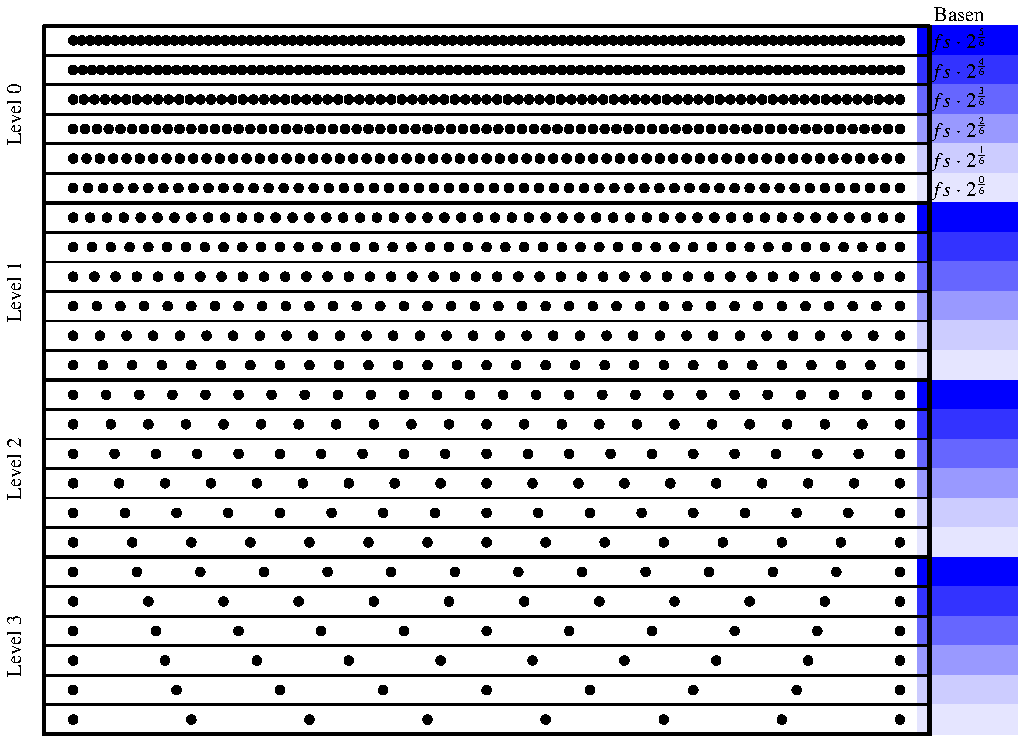
\includegraphics[width=\linewidth]{papers/autotune/sections/frames/images/msa/msa.pdf}
	\caption{Prinzip Stacked-Frame-Multiskalenanalyse mit 6 Basen und 4 Level}\label{fig:Stacked_frame}
\end{figure}%

\newpage


\subsubsection{Overlaid-Frame}

Beim Overlaid-Frame werden die einzelnen Levels übereinander gelegt. Dabei muss beachtet werden, dass die Levels verschiedener Basen in der Frequenzachse verschoben zueinander sind. Diese Verschiebung ist von $k$ abhängig. Der Verschiebungsfaktor $m$ ist entsprechend durch
\[
m= \frac{1}{k}
\]
gegeben. Die verschobenen und übereinander gelegten Levels werden alle aufaddiert. Dieser Vorgang ist in der Abbildung \ref{fig:Overlaid_frame} ersichtlich. Dabei wurde für die Grafik ein Frame mit folgenden Eigenschaften analysiert:
\[ 
f_{g}=16\text{[Hz]}; \qquad
k = 3; \qquad
\text{Level} = 3; 
\]

\begin{figure}[!ht]
	\centering
	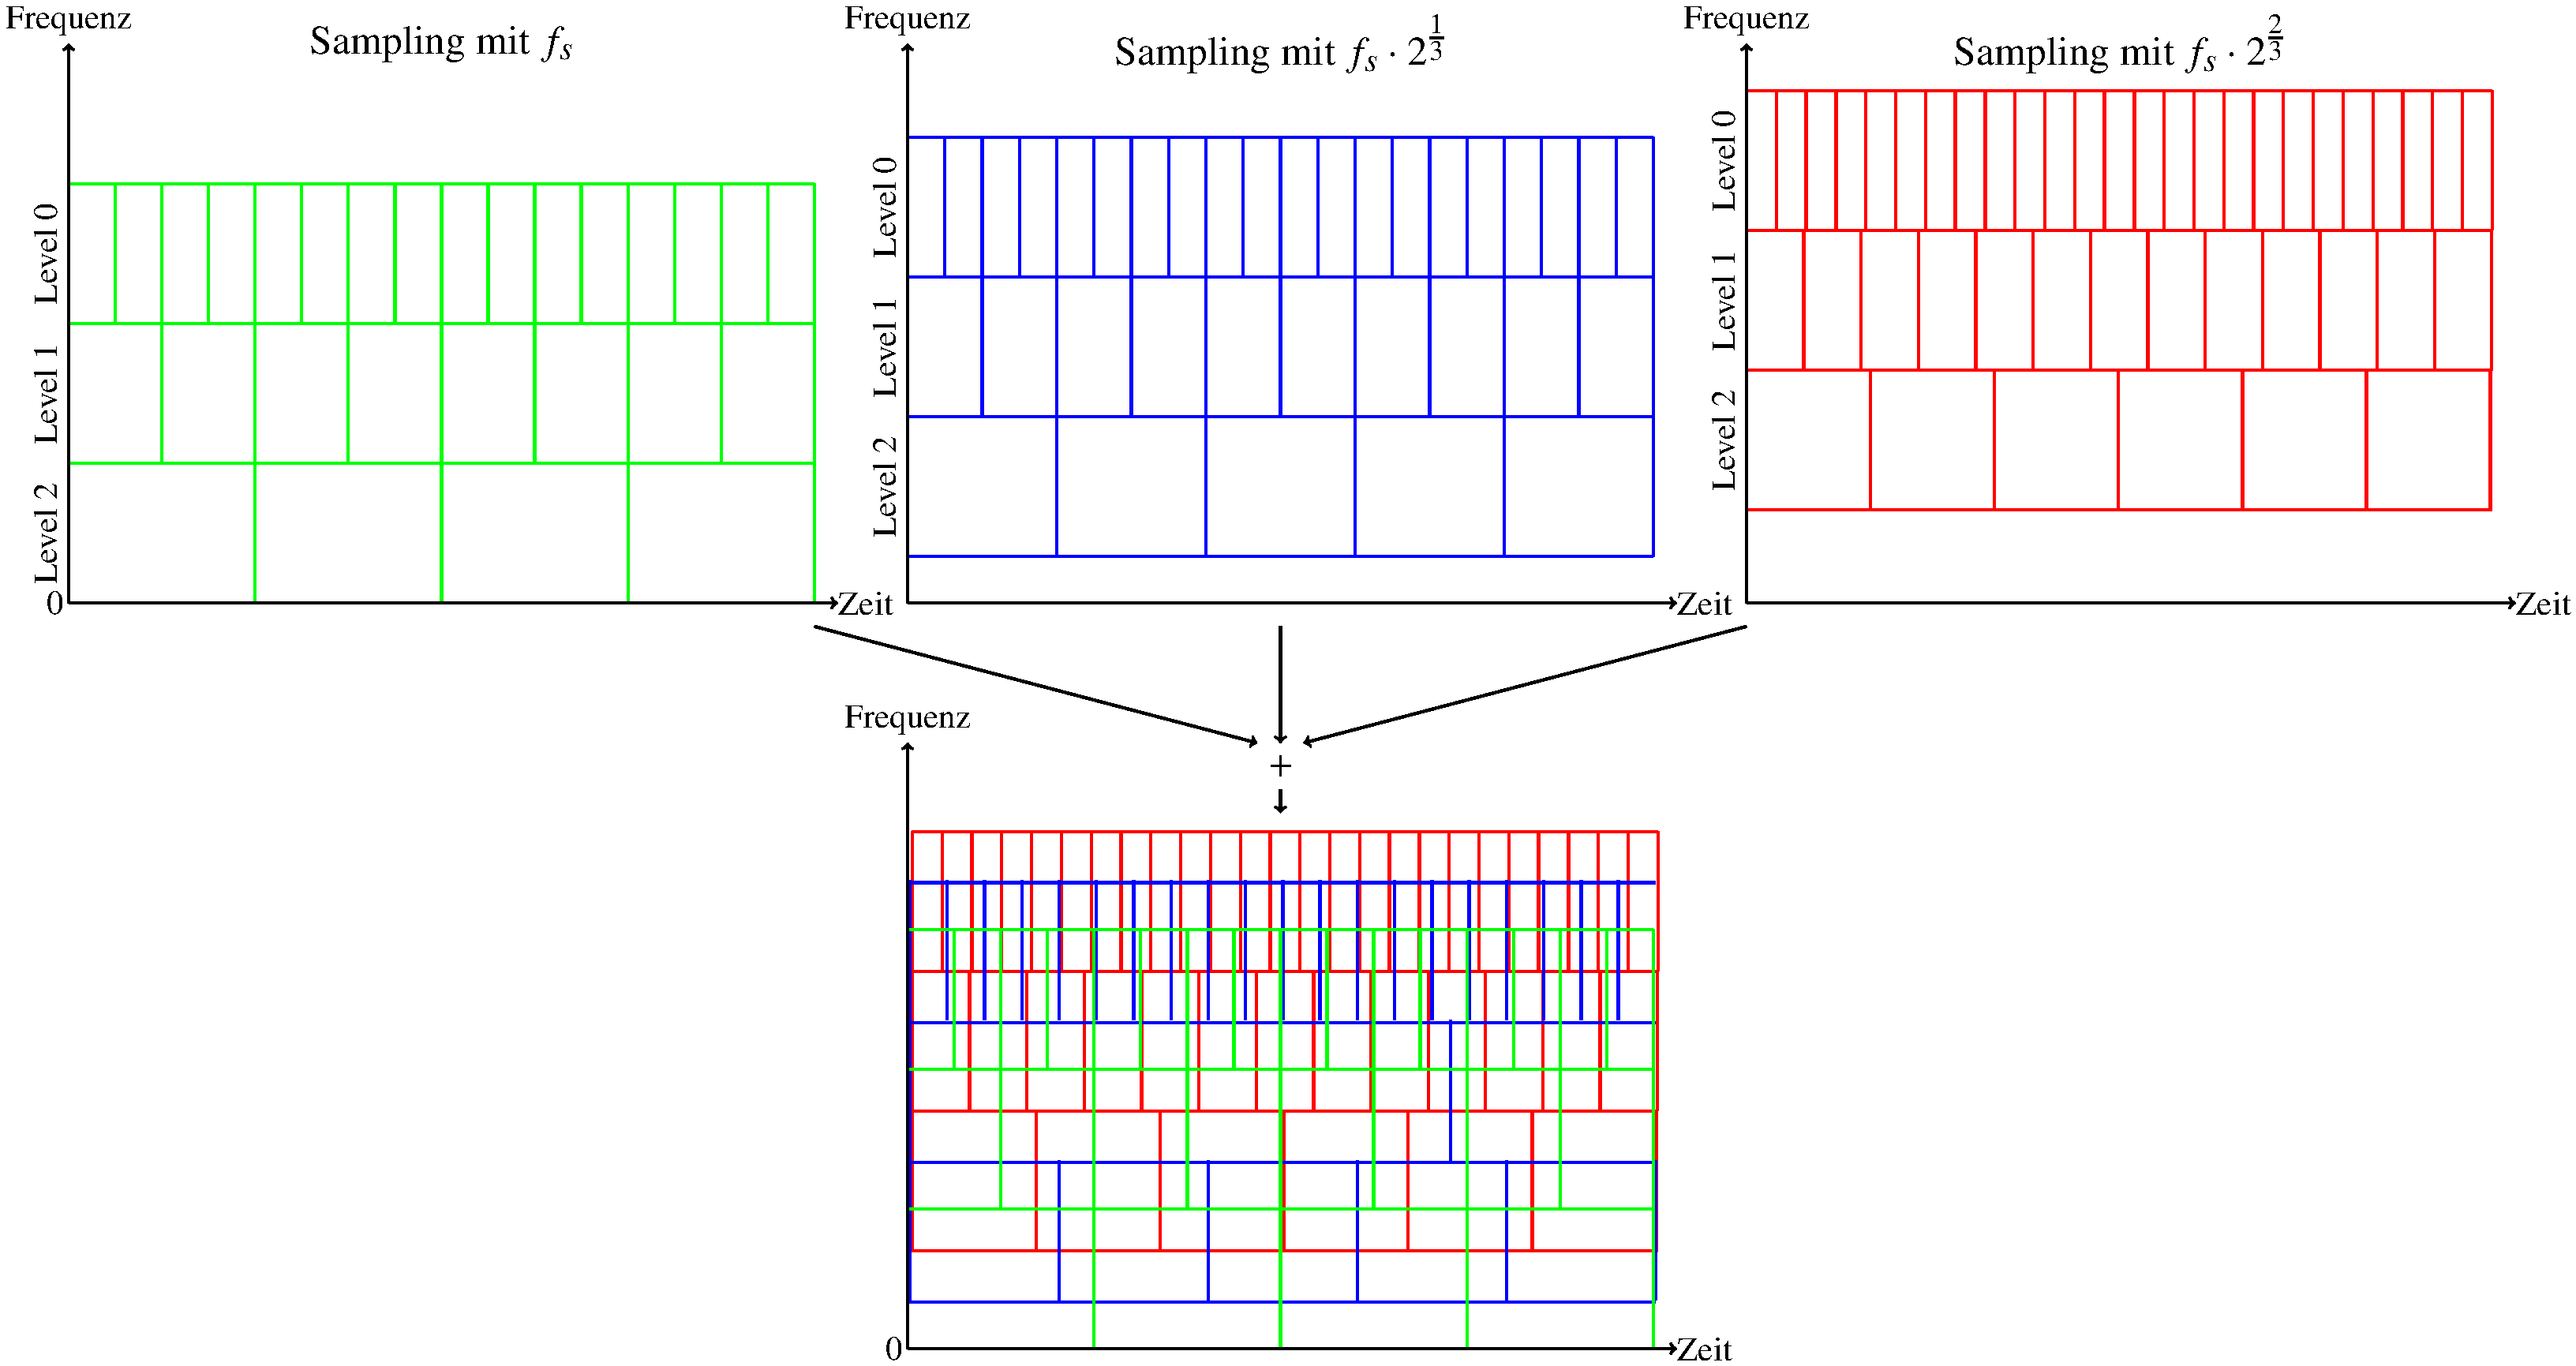
\includegraphics[width=\linewidth]{papers/autotune/sections/frames/images/frame/msa.pdf}
	\caption{Prinzip Overlaid-Frame-Multiskalenanalyse mit 3 Basen und 3 Level}\label{fig:Overlaid_frame}
\end{figure}%


Mit diesen zwei Analysearten wurden dann die folgenden Analysen durchgeführt.
\newpage

\subsection{Analyse mit Frames}

Um die verschiedenen Analyse- und Auswertungsarten vergleichen zu können, wurde ein Testsignal erstellt. Dabei sollte das Testsignal aufzeigen können ob die Analyseart zwei Halbtöne unterscheiden kann oder nicht. Mit diesem Ziel wurde folgendes Testsignal $x_{\text{Test}}$ implementiert.

\begin{loesung}
	\begin{align*}
	0 \leq t \leq 0.1\text{s} \qquad			& = \qquad (-0.5\cdot \cos(20\cdot\pi t))\cdot \sin(110\cdot 2\pi t) \\
	0.1\text{s} \leq t \leq 0.2\text{s}\qquad	& = \qquad (-0.5\cdot \cos(20\cdot\pi t))\cdot \sin(110\cdot 2\pi t) \\
	0.2\text{s} \leq t \leq 0.3\text{s}\qquad	& = \qquad 0\\
	0.3\text{s} \leq t \leq 0.4\text{s}\qquad	& = \qquad (-0.5\cdot \cos(20\cdot\pi t))\cdot \sin(220\cdot  2^{\frac{1}{12}}\cdot 2\pi t) \\
	0.4\text{s} \leq t \leq 0.5\text{s}\qquad	& = \qquad (-0.5\cdot \cos(20\cdot\pi t))\cdot \sin(220\cdot2^{\frac{2}{12}}\cdot 2\pi t) \\
	0.5\text{s} \leq t \leq 0.6\text{s}\qquad	& = \qquad 0 \\
	0.6\text{s} \leq t \leq 0.7\text{s}\qquad	& = \qquad (-0.5\cdot \cos(10\cdot\pi t))\cdot \sin(220\cdot2^{\frac{2}{12}}\cdot 2\pi t) \\
	0.7\text{s} \leq t \leq 0.8\text{s}\qquad	& = \qquad \sin(220\cdot2^{\frac{5}{12}}\cdot 2\pi t) \\
	0.8\text{s} \leq t \leq 0.9\text{s}\qquad	& = \qquad \sin(220\cdot2^{\frac{6}{12}}\cdot 2\pi t) \\
	0.9\text{s} \leq t \leq 1\text{s}\qquad		& = \qquad (-0.5\cdot \cos(10\cdot\pi t))\cdot \sin(220\cdot2^{\frac{6}{12}}\cdot 2\pi t) \\
	\end{align*}
\end{loesung}
Das Testsignal ist auch in der folgenden Abbildung\ref{fig:frame-testsig} dargestellt.
\begin{figure}[!ht]
	\centering
	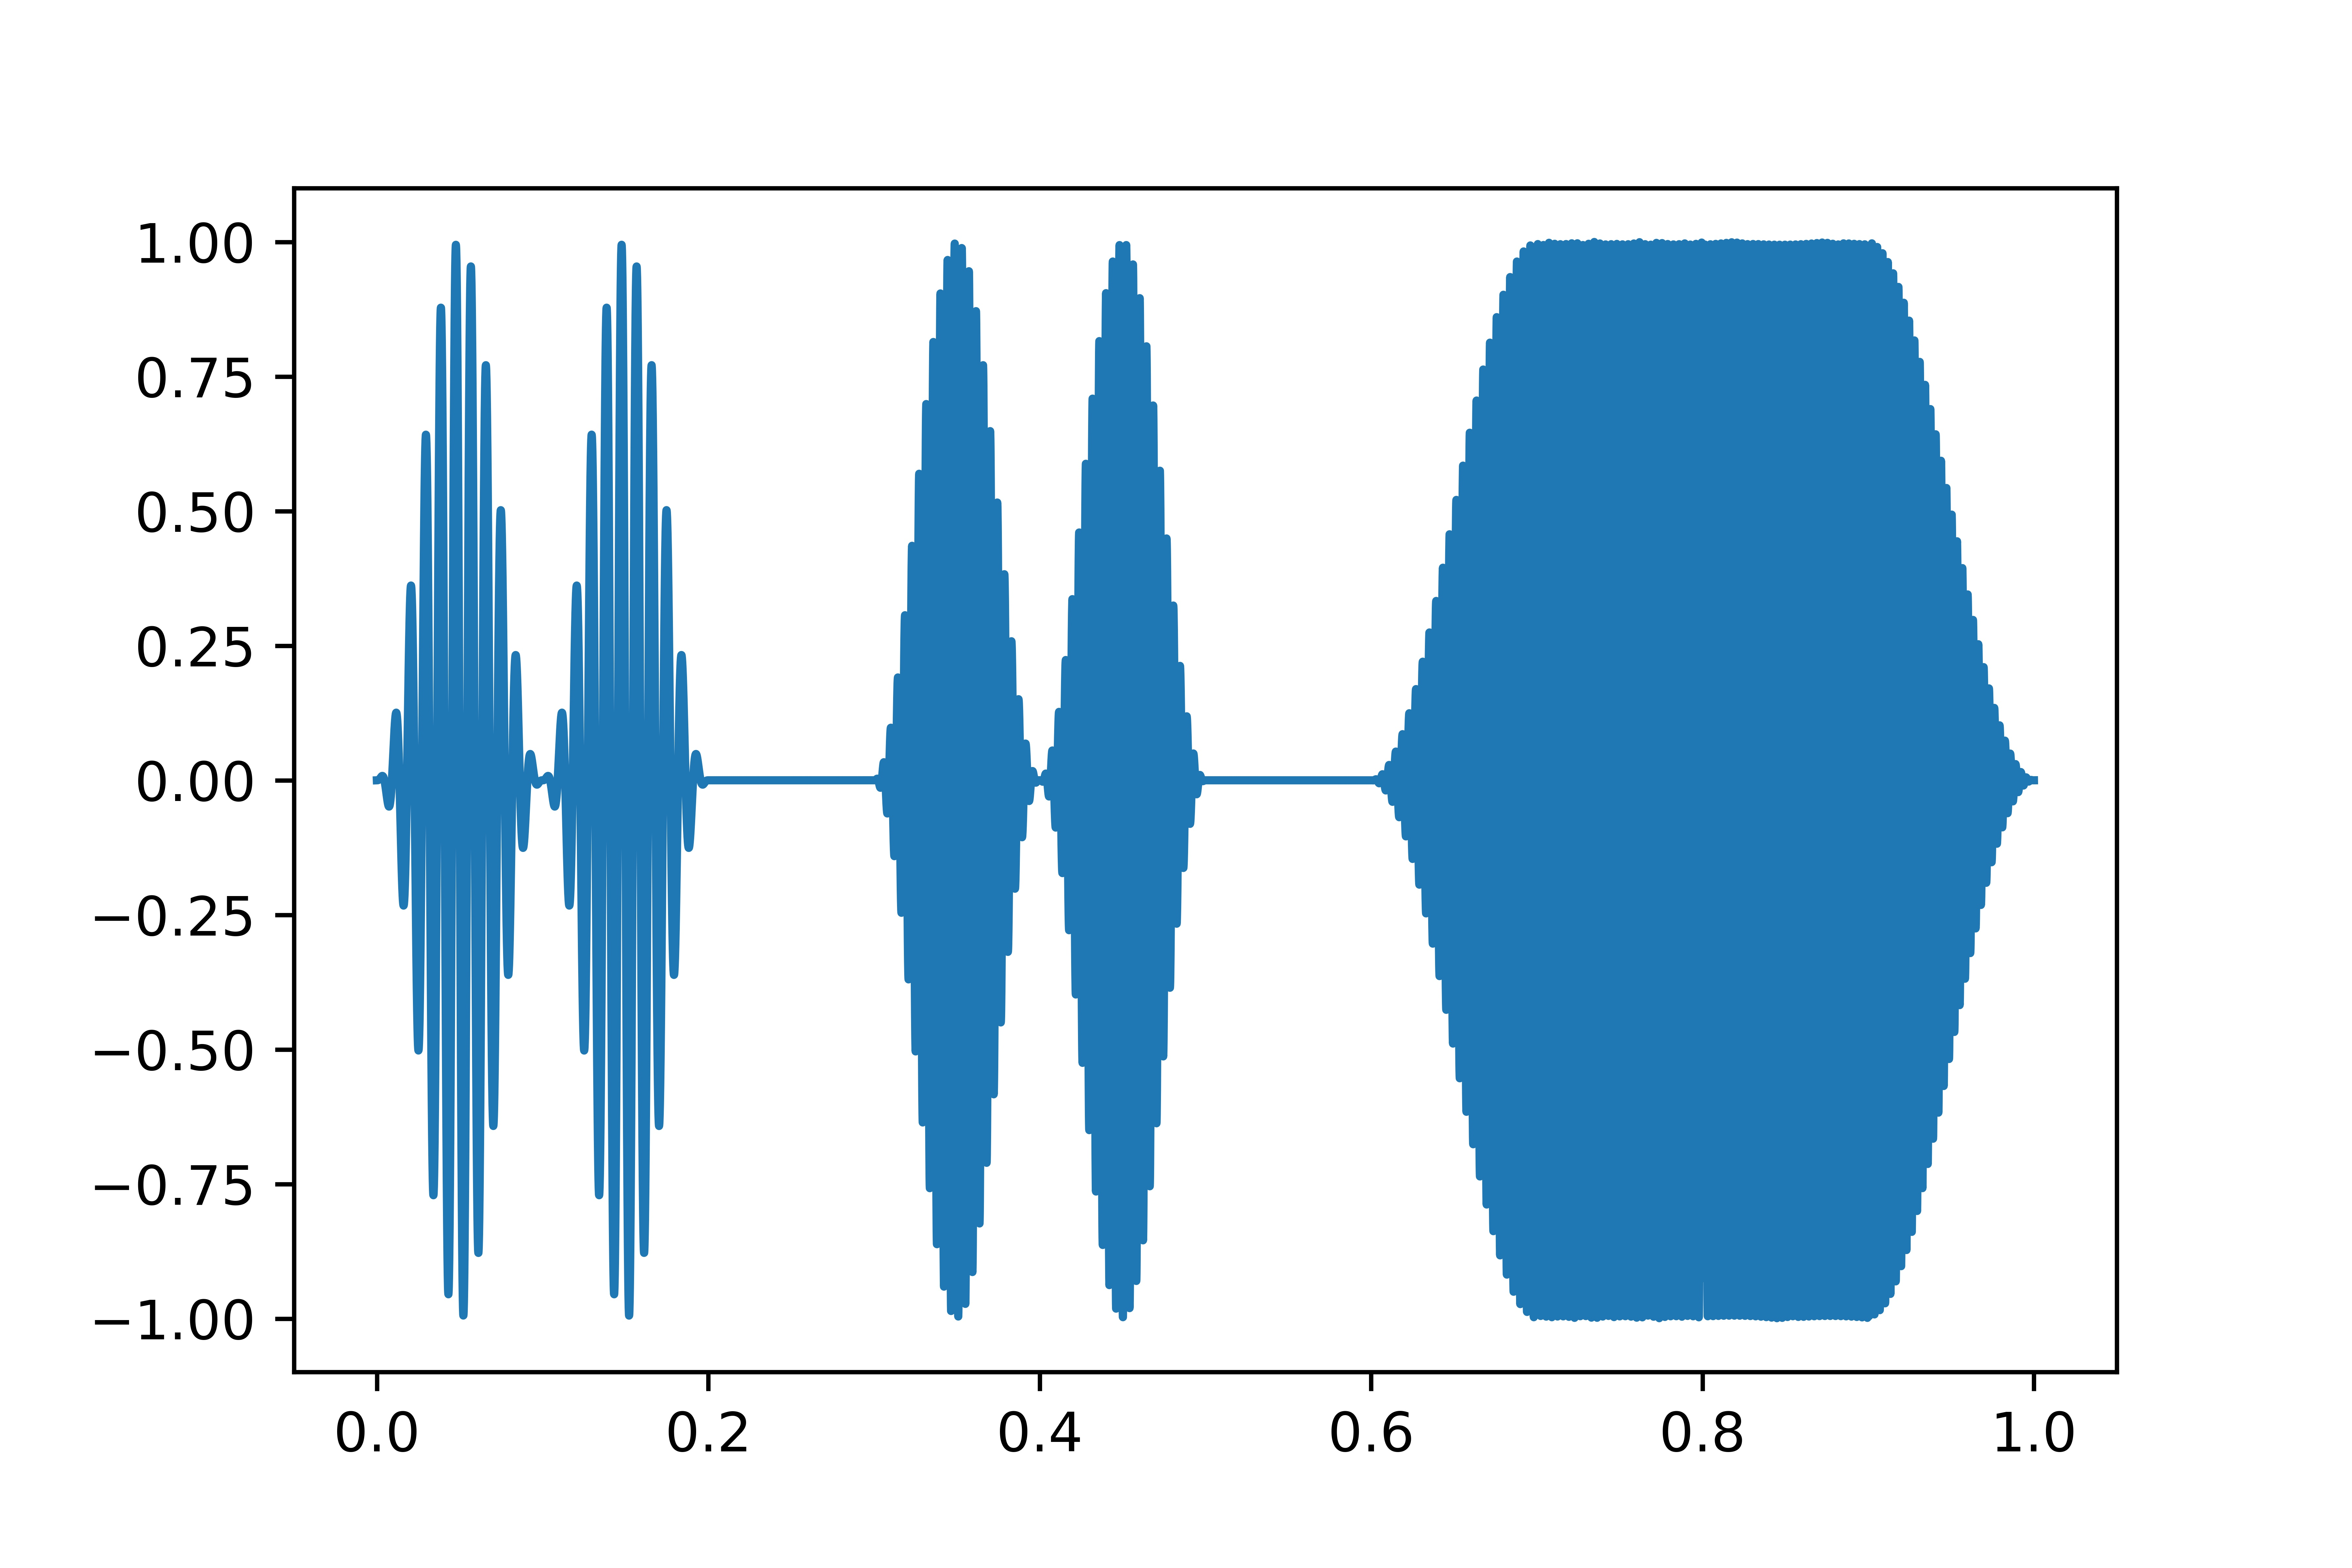
\includegraphics[width=0.9\columnwidth]{papers/autotune/sections/frames/images/testsig.jpg}
	\captionof{figure}{Testsignal $x_{\text{Test}}$}\label{fig:frame-testsig}
\end{figure}%

Auf $x_{\text{Test}}$ wurde wieder die gleiche cwt mit komplexen Gauss Wavelet angewendet. Dieses Resultat soll als Referenz dienen, um die Frame-Analysen zu vergleichen.
\\
In den Grafiken \ref{fig:frame-cwt} und \ref{fig:stacked-12dwt} wird eine Stacked-Frame-Analyse \ref{fig:stacked-12dwt} mit 12 Basen und eine cwt-Analyse \ref{fig:frame-cwt} des $x_{\text{Test}}$ \ref{fig:frame-testsig} nebeneinander gestellt. Die beiden Resultate werden dabei nur in Absolutwerten dargestellt, da so die Resultate noch eindeutiger sind. Die Stacked-Frame-Analyse hat deutliche Peak- und Nullstellen an Orten wo die cwt keine solcher Artefakte aufweist. Diese sind durch die verschiebung der Level erklärbar. Diese Musterung ist jedoch schon in der Abbildung \ref{fig:Stacked_frame} erahnbar.    
\begin{figure}[!ht]
	\centering
	\begin{tabularx}{\columnwidth}{XX}
		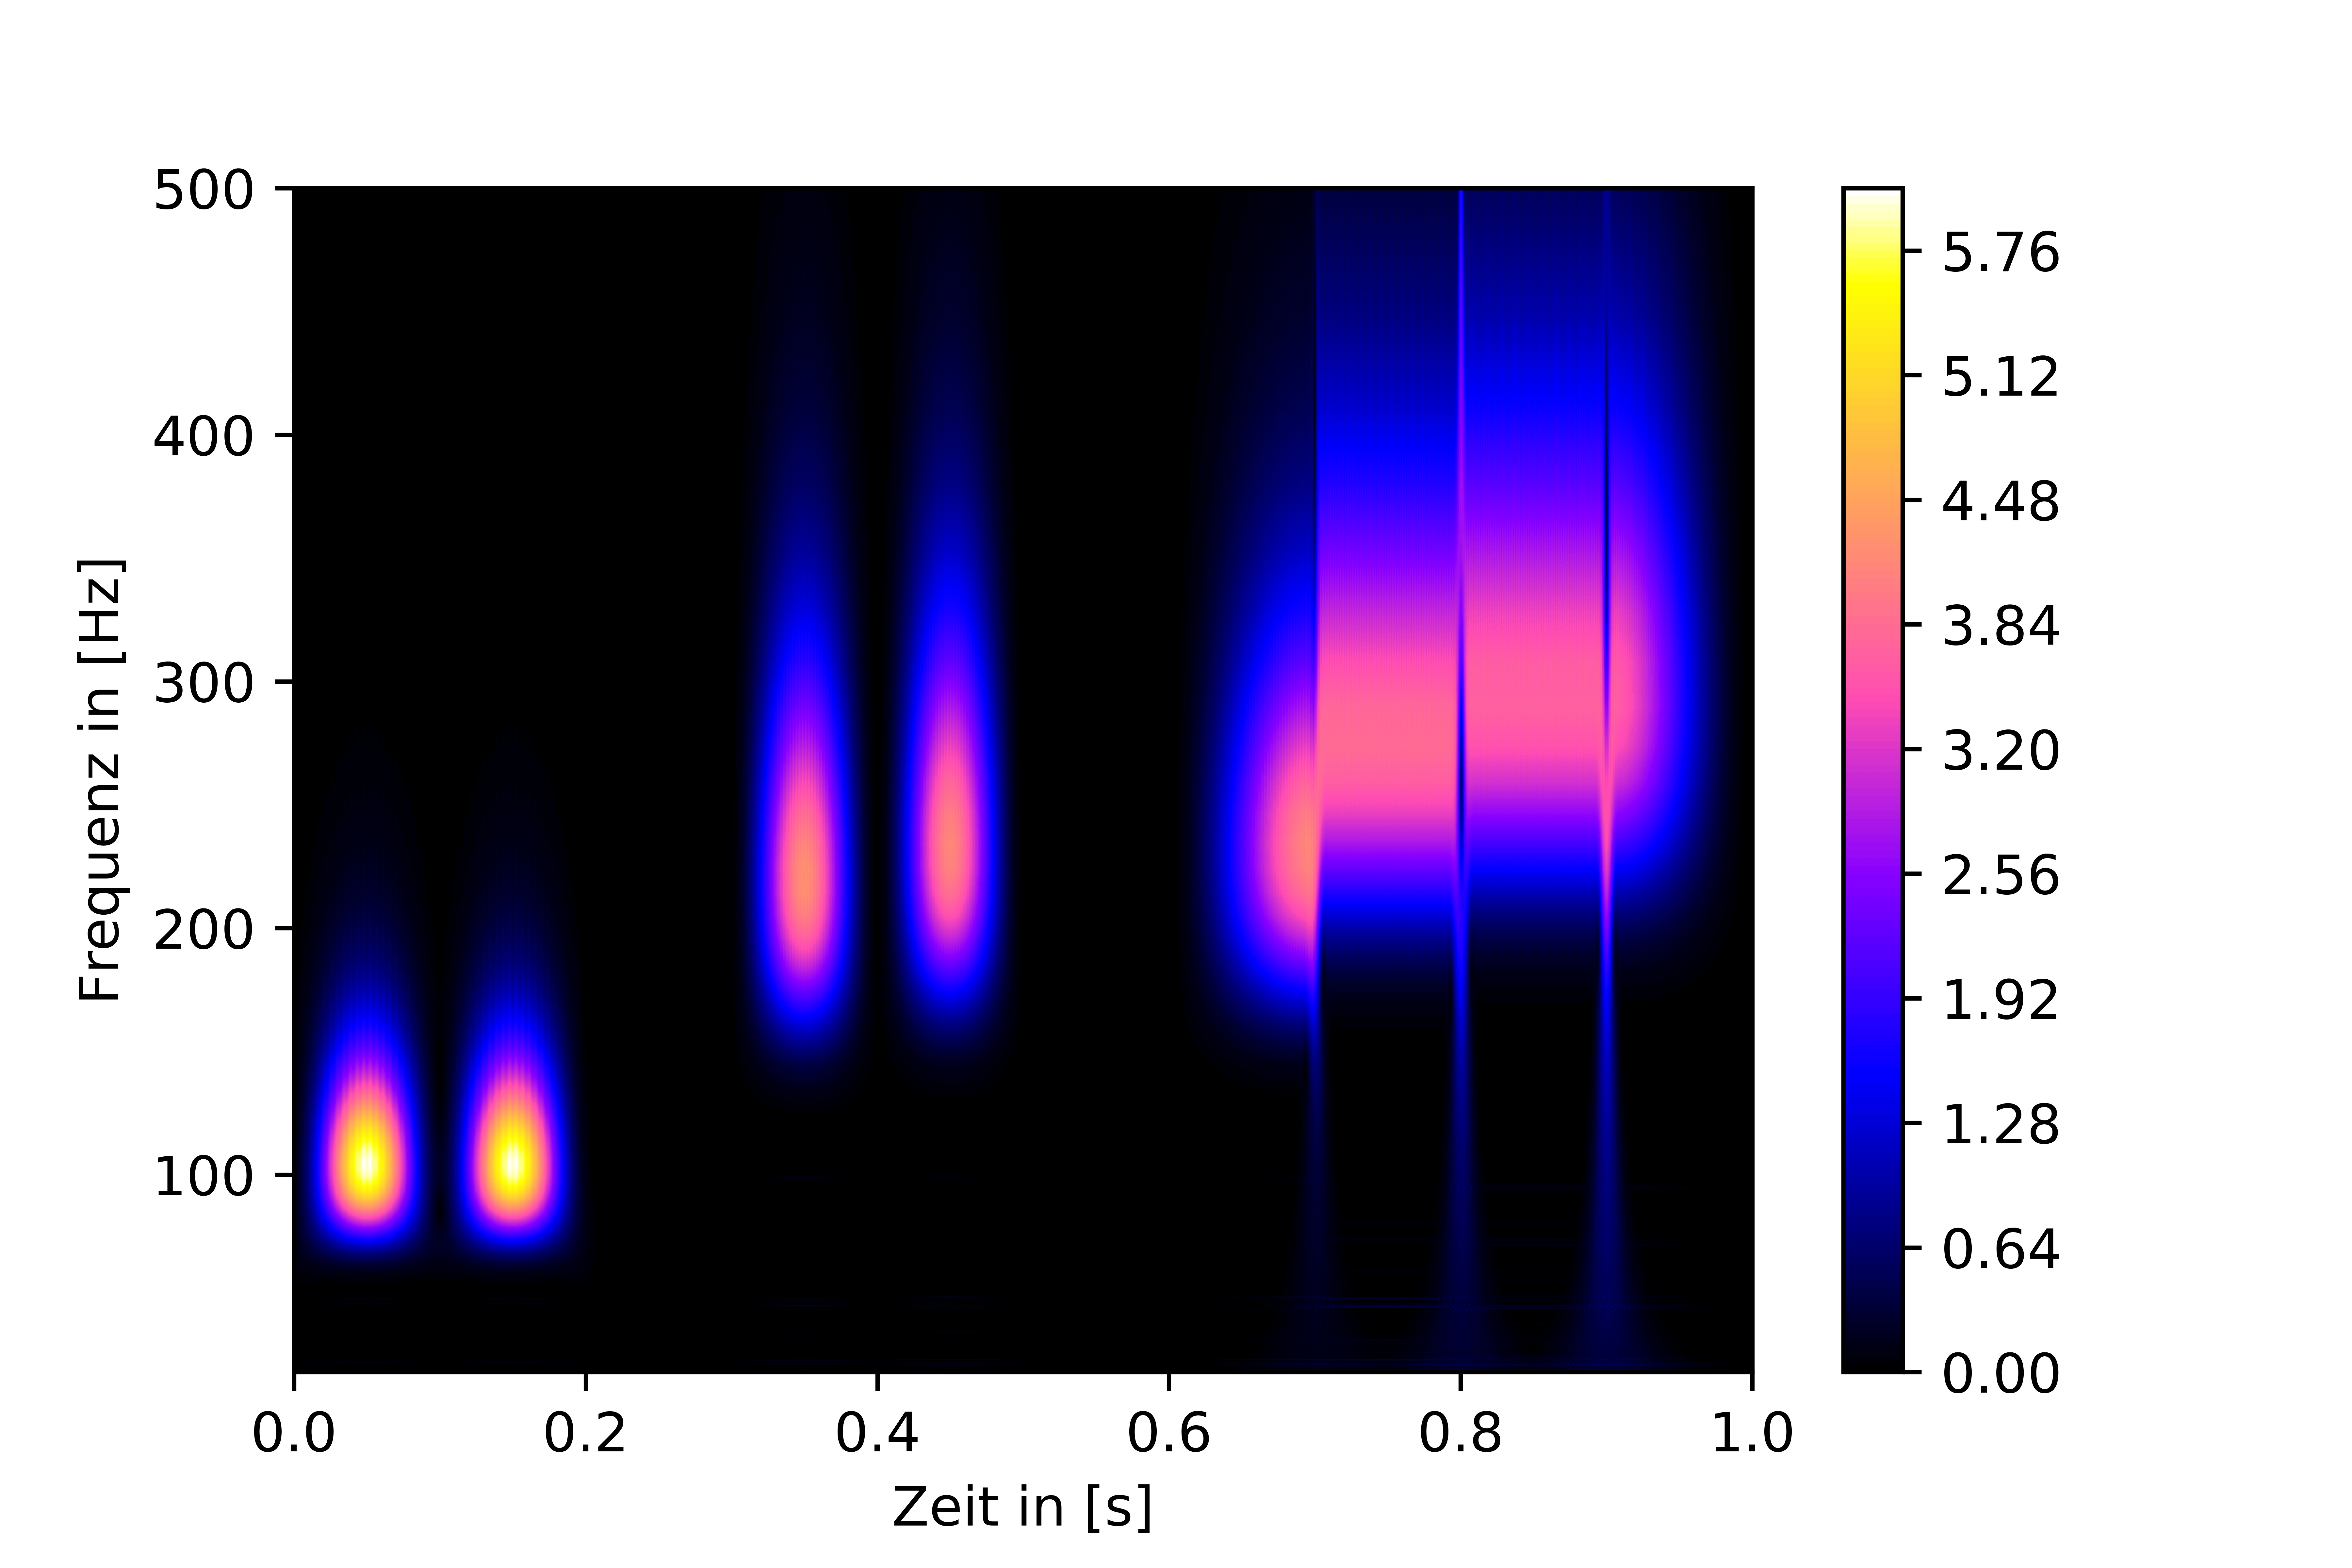
\includegraphics[width=1.3\linewidth]{papers/autotune/sections/frames/images/cwt.jpg}
		\captionof{figure}{Cwt Analyse mit komplexem Gauss Wavelet des Testsignals}\label{fig:frame-cwt}
		&   \includegraphics[width=1.3\linewidth]{papers/autotune/sections/frames/images/Stacked/12dwt.jpg}   
		\captionof{figure}{Stacked-Frame-Analyse mit Daubechies 8 Wavelet $k=12$}\label{fig:stacked-12dwt}         
	\end{tabularx}
\end{figure}%

Um den gleichen Vergleich für die Overlaid-Frame-Analyse zu haben wurde in der Grafiken \ref{fig:frame-cwt} und \ref{fig:overlaid-12dwt} eine Overlaid-Frame-Analyse mit 12 Basen \ref{fig:overlaid-12dwt} und eine cwt-Analyse \ref{fig:frame-cwt2} des $x_{\text{Test}}$ \ref{fig:frame-testsig} nebeneinander gestellt. Die Overlaid-Frame-Analyse sieht der cwt ungemein ähnlich. Im Vergleich mit der Stacked-Frame-Analyse besitzt sie auch nicht diese Artifakte der Levels. Der Unterschied zur cwt ist aber noch leicht sichtbar. In der Zeitachse gibt es immer wieder Störungen und auch in der Frequenzachse ist das Resultat ein wenig verzerrt. \\
 

\begin{figure}[!ht]
	\centering
	\begin{tabularx}{\columnwidth}{XX}
		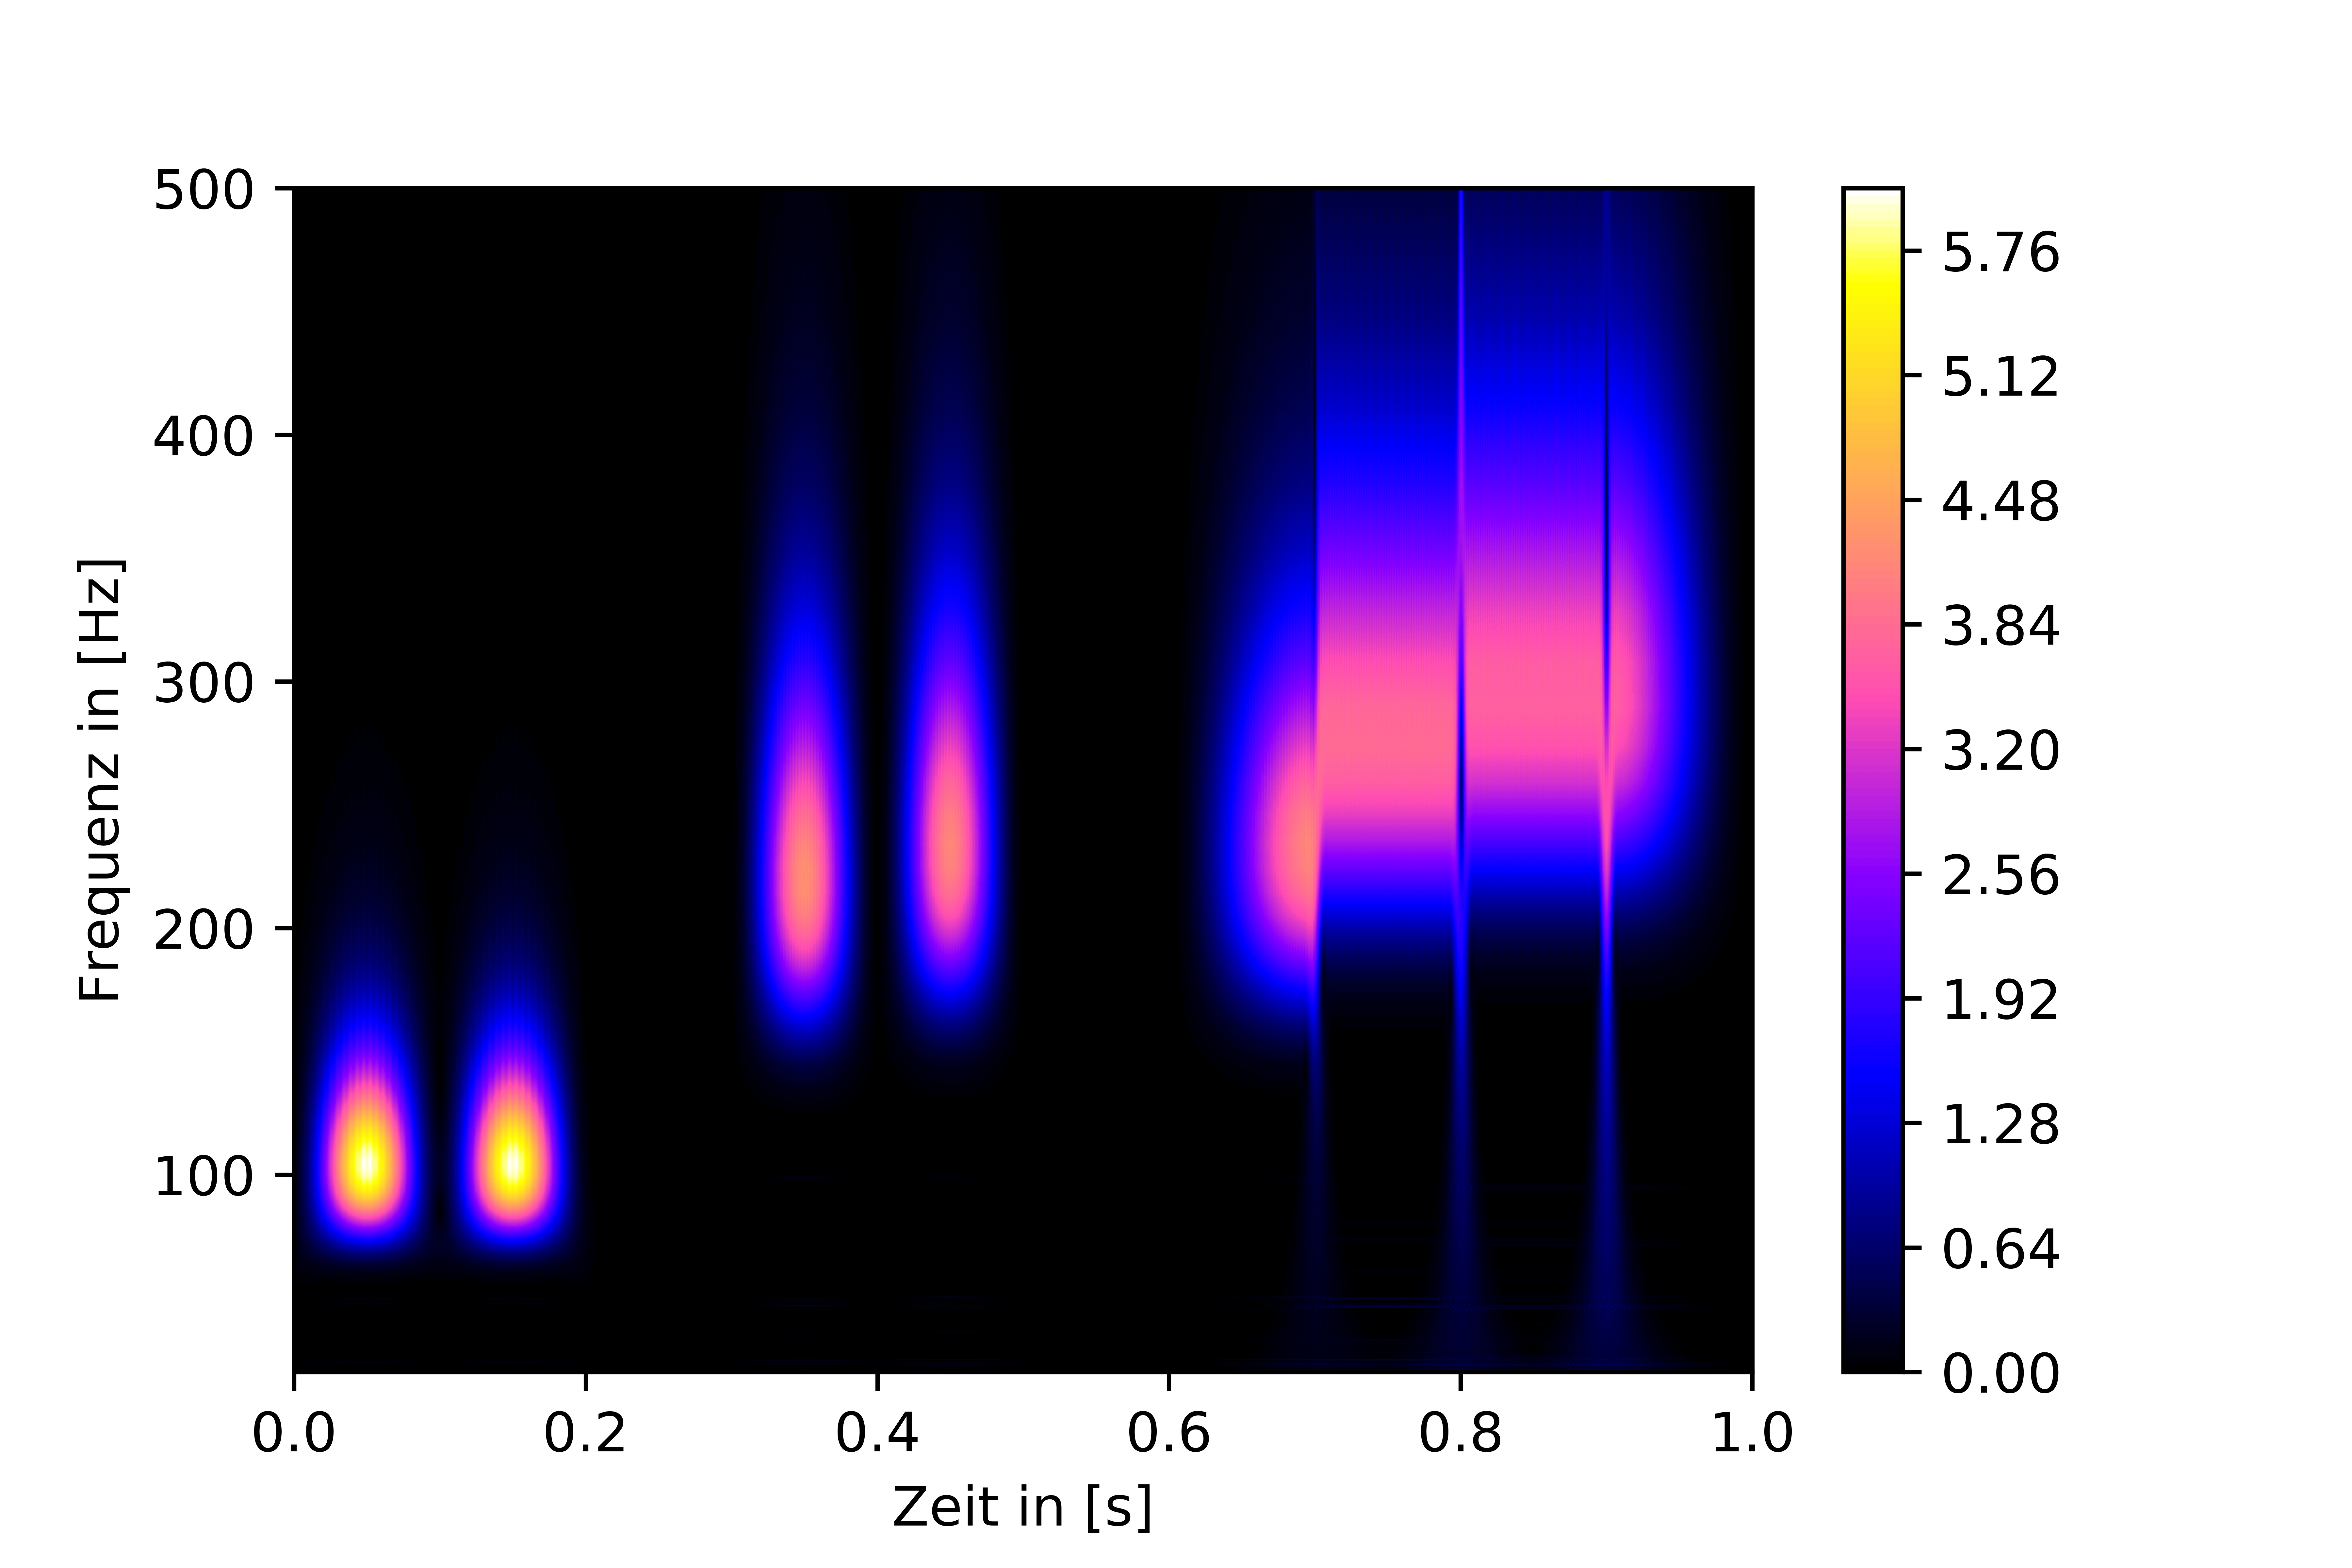
\includegraphics[width=1.3\linewidth]{papers/autotune/sections/frames/images/cwt.jpg}
		\captionof{figure}{Cwt Analyse mit komplexem Gauss Wavelet des Testsignals}\label{fig:frame-cwt2}
		&   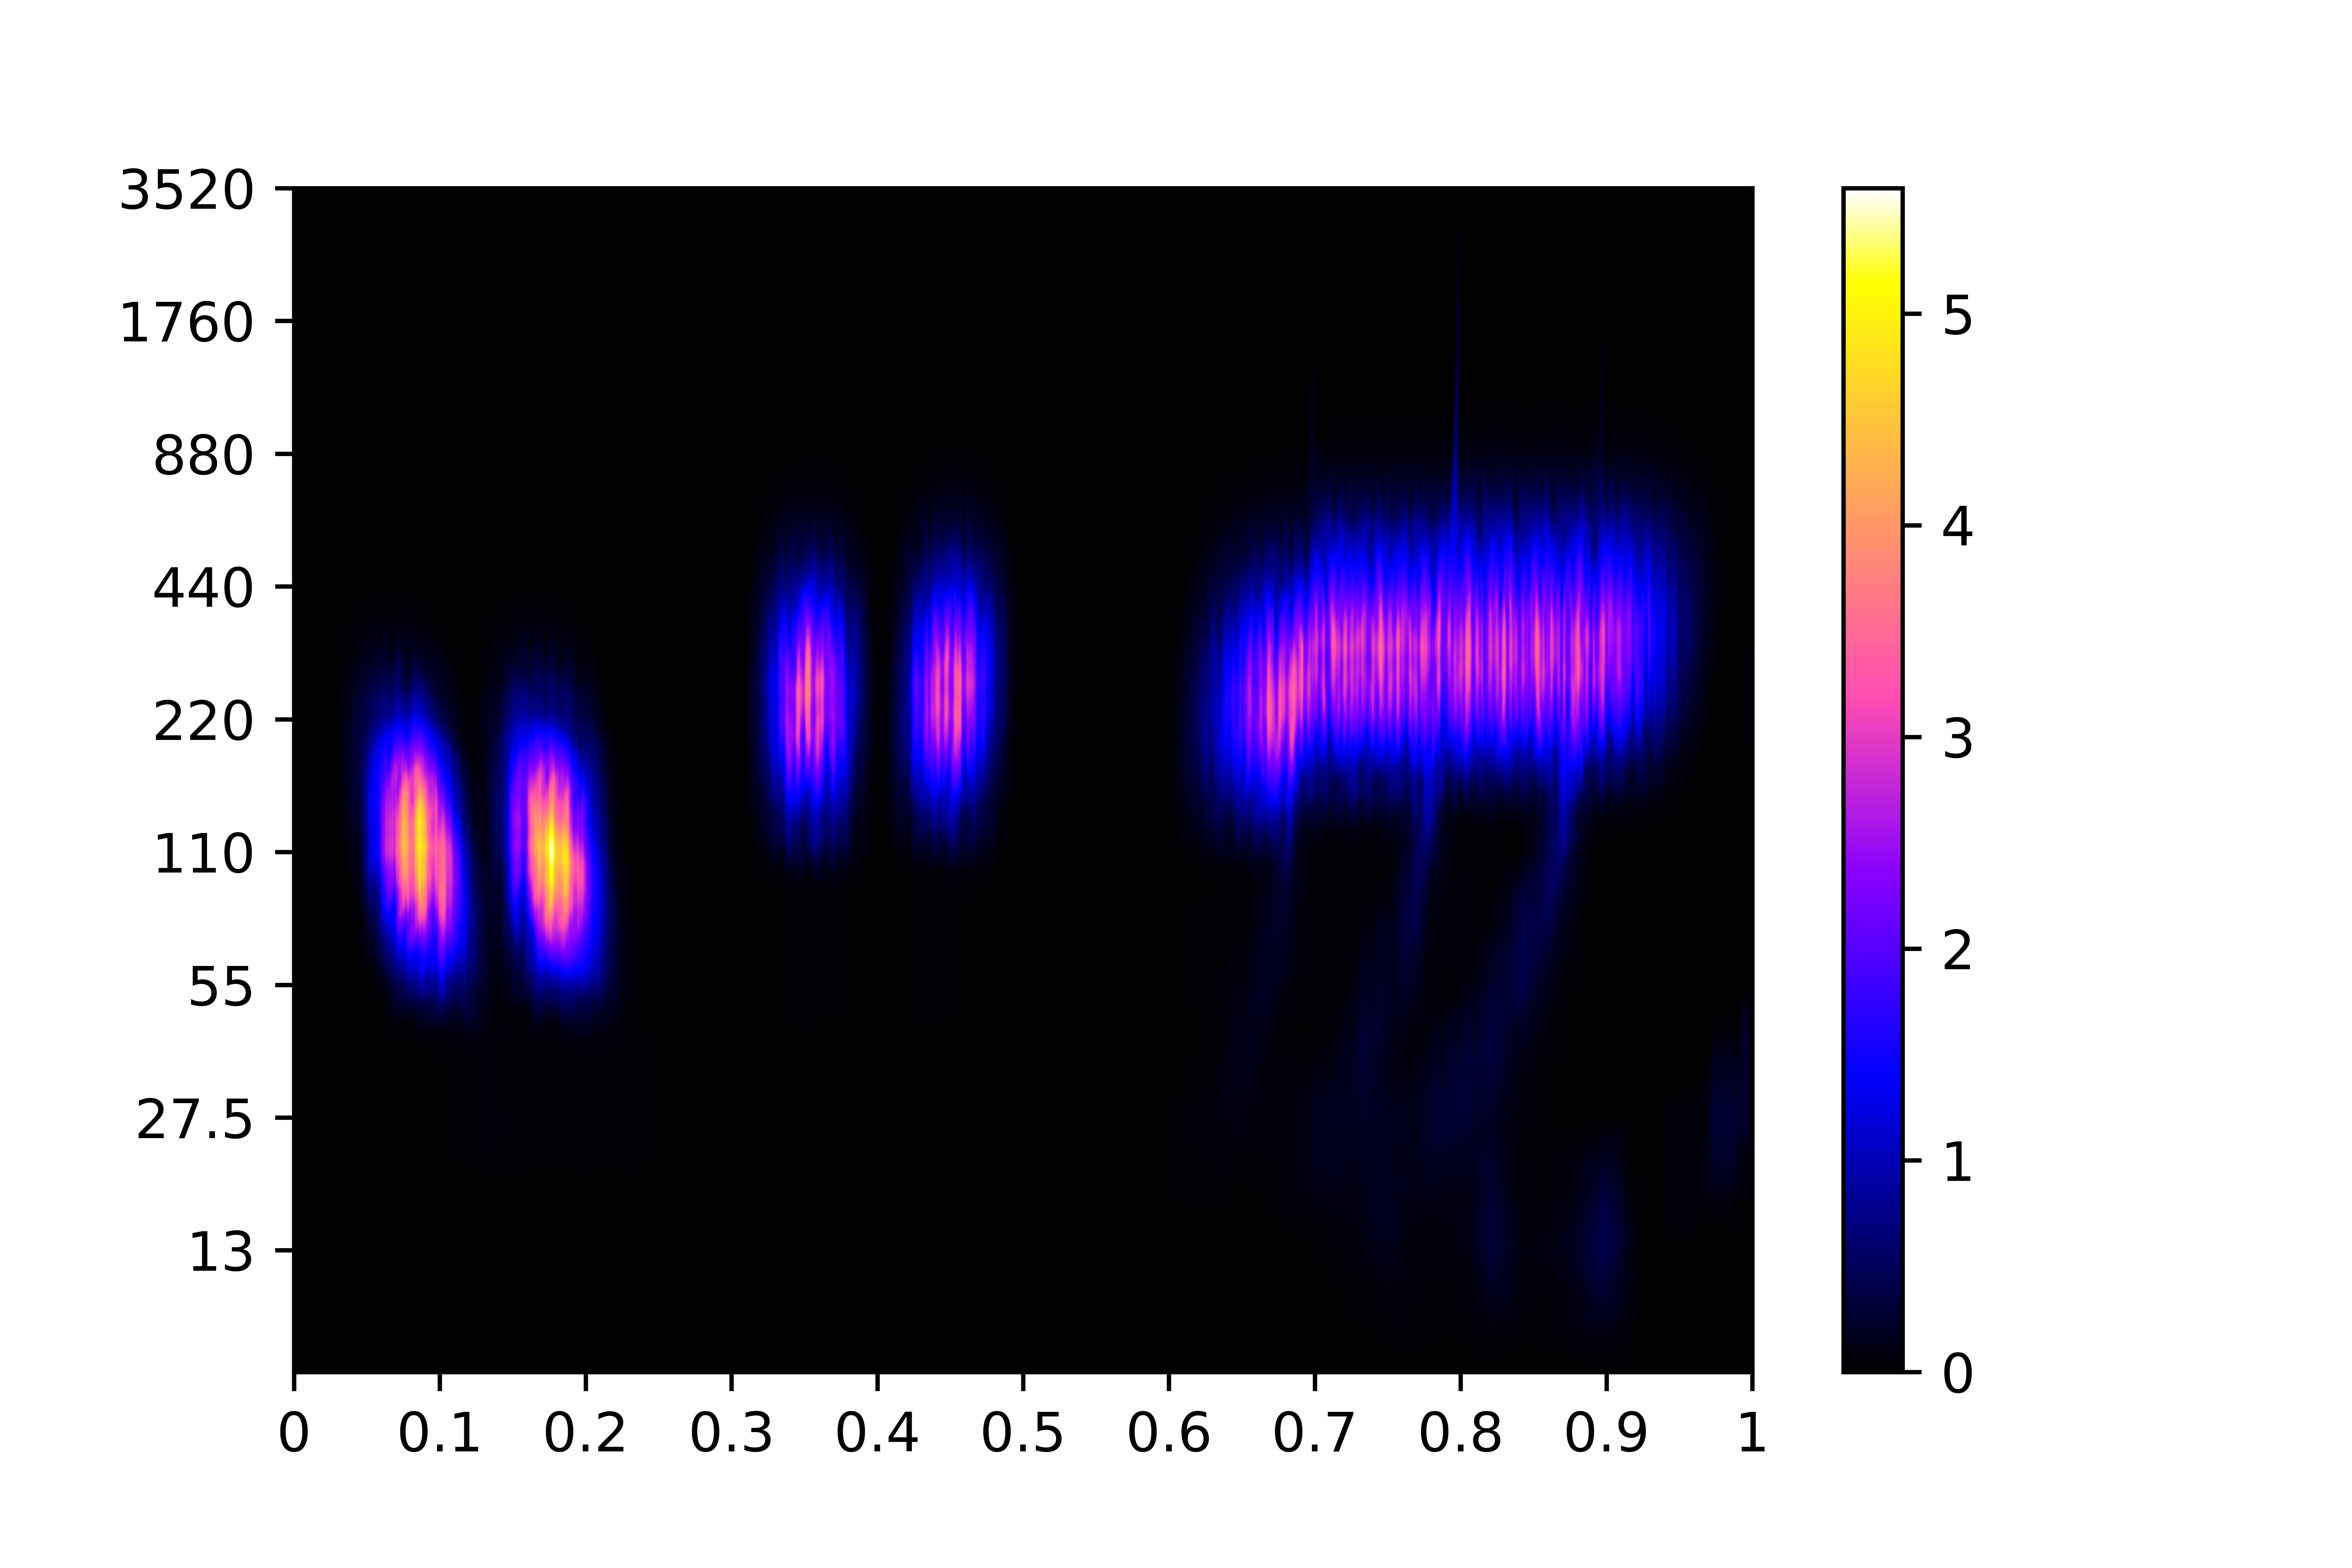
\includegraphics[width=1.3\linewidth]{papers/autotune/sections/frames/images/Overlaid/7040Hz12dwt.jpg}   
		\captionof{figure}{Overlaid-Frame-Analyse mit Daubechies 8 Wavelet $k=12$}\label{fig:overlaid-12dwt}         
	\end{tabularx}
\end{figure}%

\newpage

Um die Auflösung der Stacked-Frame und Overlaid-Frame zu erhöhen können jedoch einfach noch mehr Basen hinzugefügt werden. In dem folgenden Grafiken\ref{fig:Stacked-48dwt} und \ref{fig:overlaid-48dwt} wurde $k=48$ verwendet. 

\begin{figure}[!ht]
	\centering
	\begin{tabularx}{\columnwidth}{XX}
		\includegraphics[width=1.3\linewidth]{papers/autotune/sections/frames/images/Stacked/48dwt.jpg}
		\captionof{figure}{Stacked-Frame-Analyse mit Daubechies 8 Wavelet $k=48$}\label{fig:Stacked-48dwt}
		&   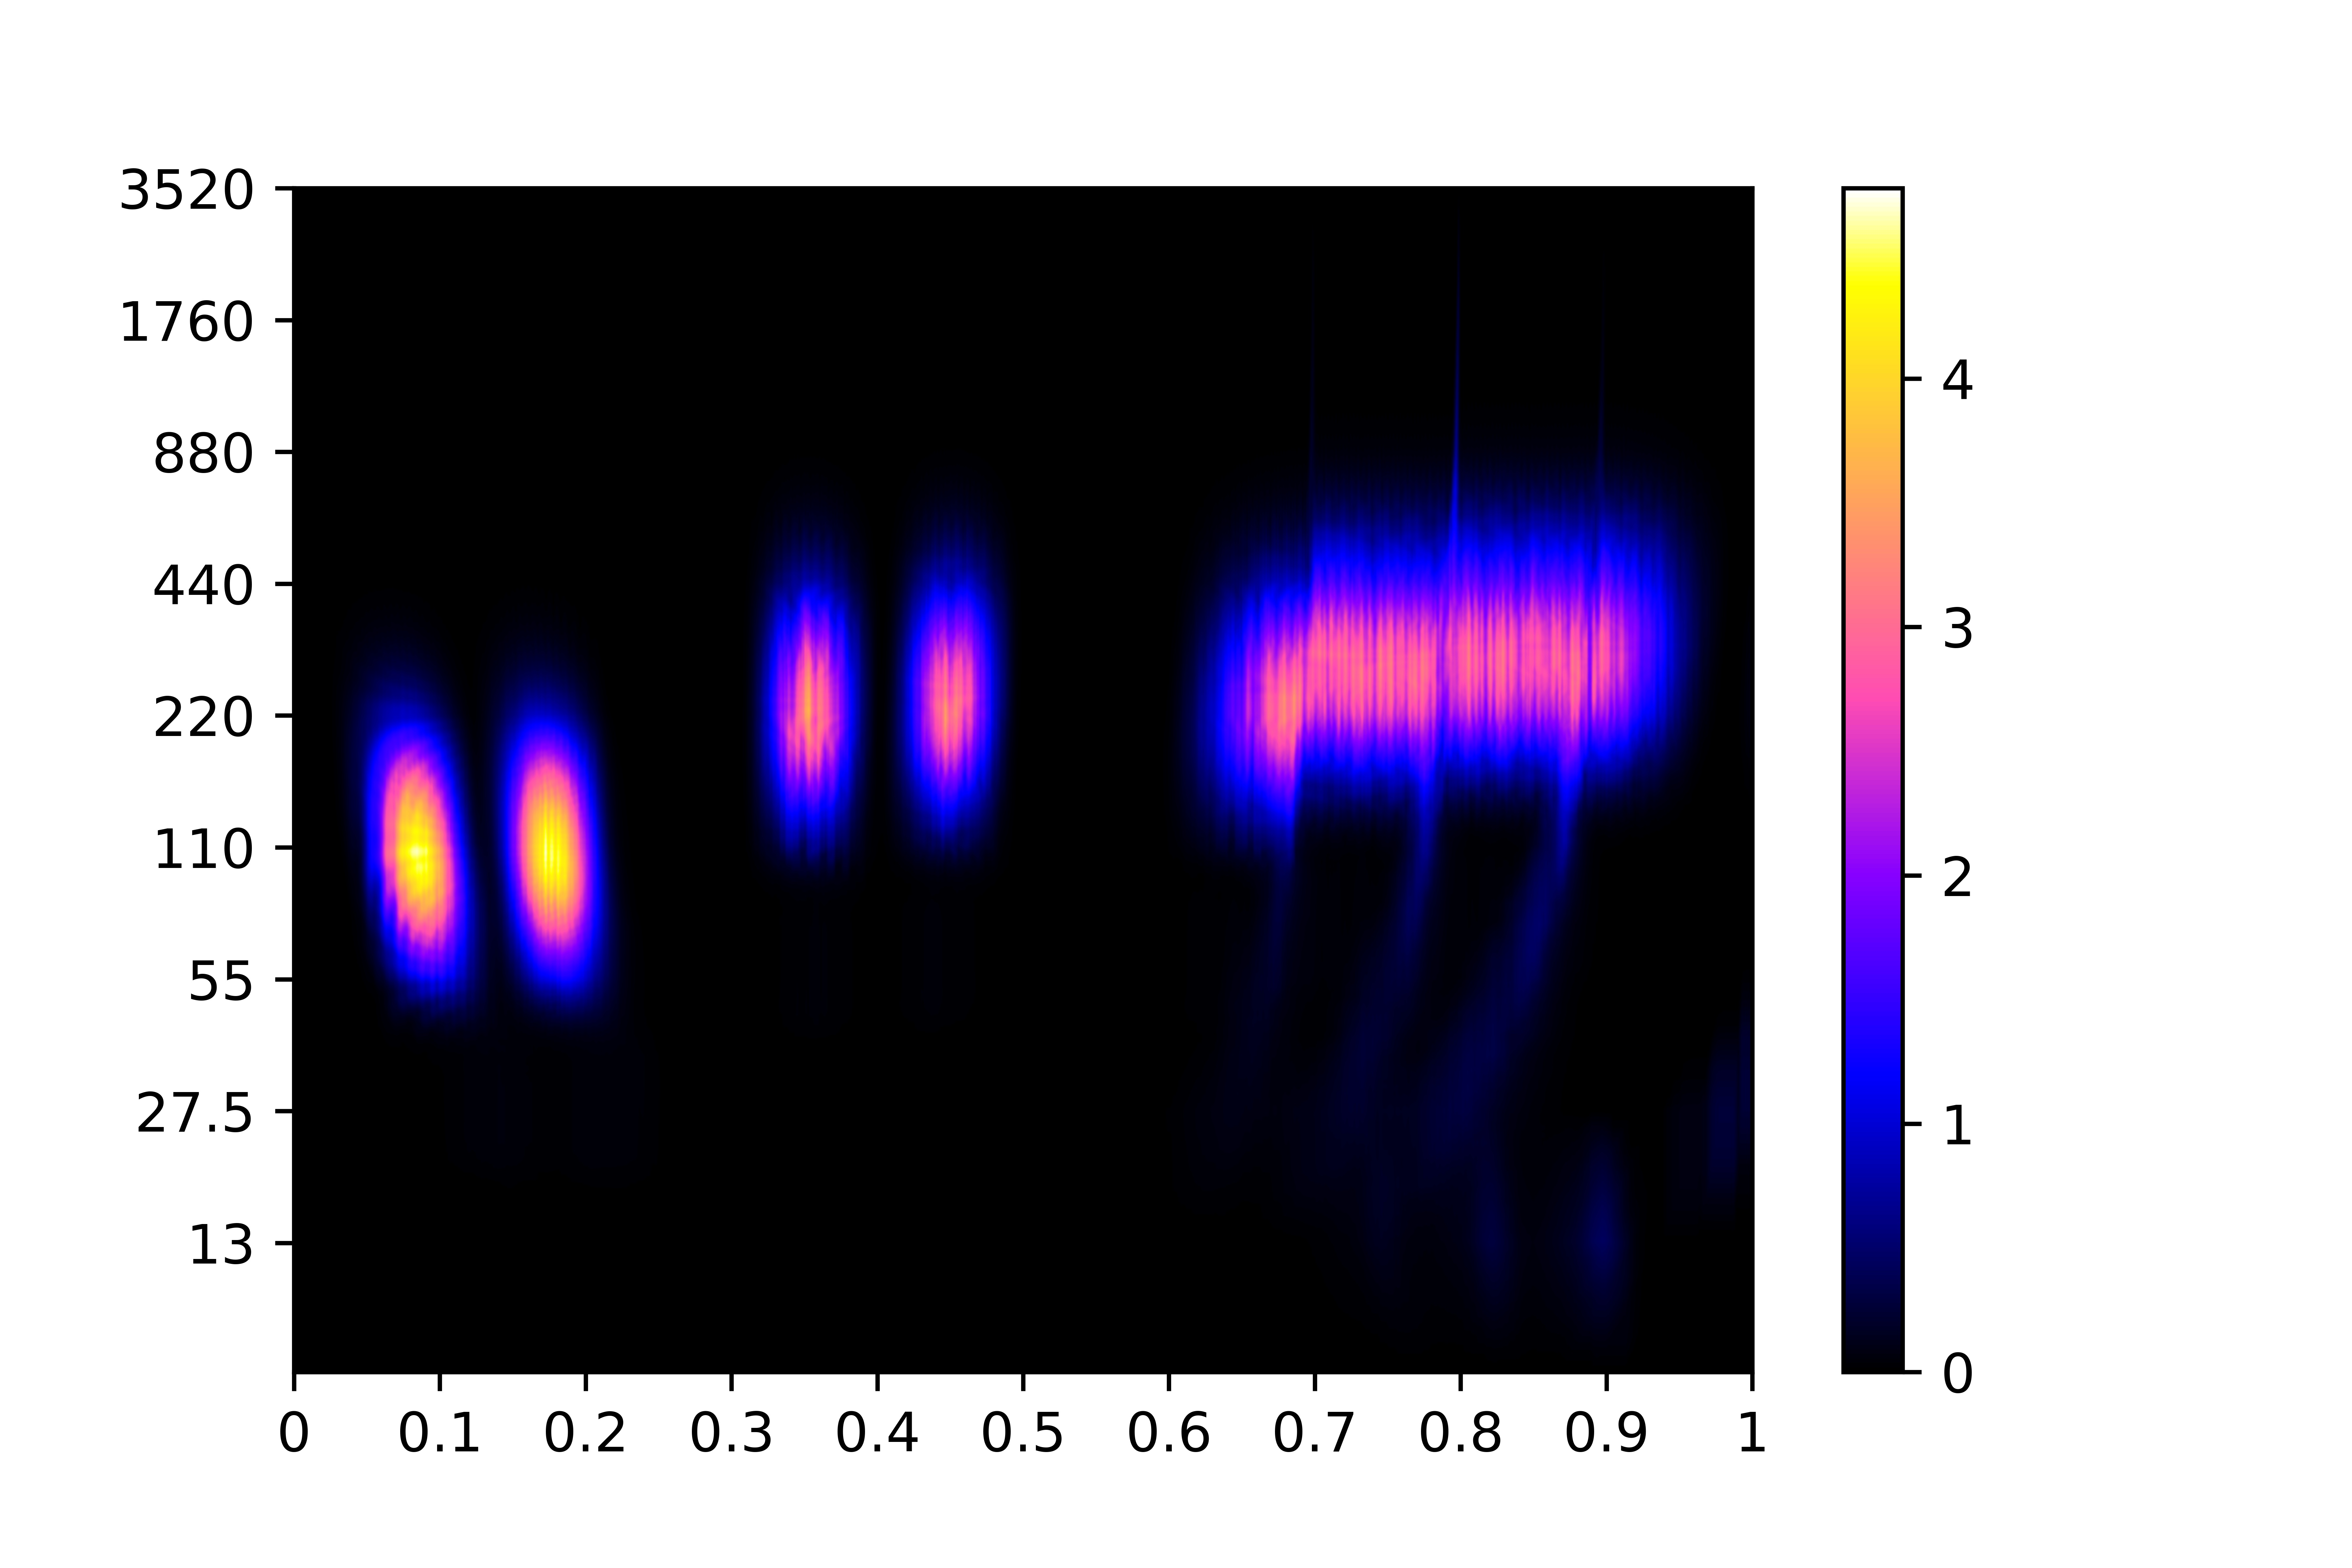
\includegraphics[width=1.3\linewidth]{papers/autotune/sections/frames/images/Overlaid/7040Hz48dwt.jpg}   
		\captionof{figure}{Overlaid-Frame-Analyse mit Daubechies 8 Wavelet $k=48$}\label{fig:overlaid-48dwt}         
	\end{tabularx}
\end{figure}%

\newpage

Von diesen Analyseresultaten sollen nun auch die Frequenzen extrahiert werden. Dabei macht man sich die lokalen Maxima der Matrix zunutze. Man vergleicht in der Matrix selbst die jeweiligen Nachbarwerte. Von den lokalen Maxima werden die Koordinaten gesammelt. Diese Koordinaten können dann mit den Level der verschiedenen Basen verglichen werden. Je nach Koordinaten höhe in der Matrix kann ein kleineres Frequenzband zugewiesen werden in welchem sich das analysierte Signal zu diesem Zeitpunkt befinden sollte. Dieses Frequenzband kann man durch die Anzahl Basen $k$  und das gegebene Level wieder rekonstruieren.\\

Um eine bessere Qualität von Maximalstellen zu erhalten, kann noch ein Maximum Filter auf die Matrix angewendet werden. Dieser Maximalfilter ersetzt in einem vordefinierten Radius $r$, die umliegenden Werte einer Matrix, mit dem lokal gefundenen Maximalwert. Das Ziel des Maximumfilters ist die Elimination der Nullstellen Artefakten, welche direkt in den wichtigen Signalverläufen vorkommen. Durch die Anwendung eines Maximalfilters werden jedoch auch Resultate verfälscht. Diese Verfälschung kann jedoch meistens vernachlässigt werden.\\

In der Folgenden Grafik\ref{fig:cwt_max} wurde das genannte Verfahren um Maximalstellen zu finden an der cwt Analyse angewendet. Diese kann somit als Referenz dienen wie eine Ideale Frequenzrückgewinnung aussehen kann. 

\begin{figure}[!ht]
	\centering
	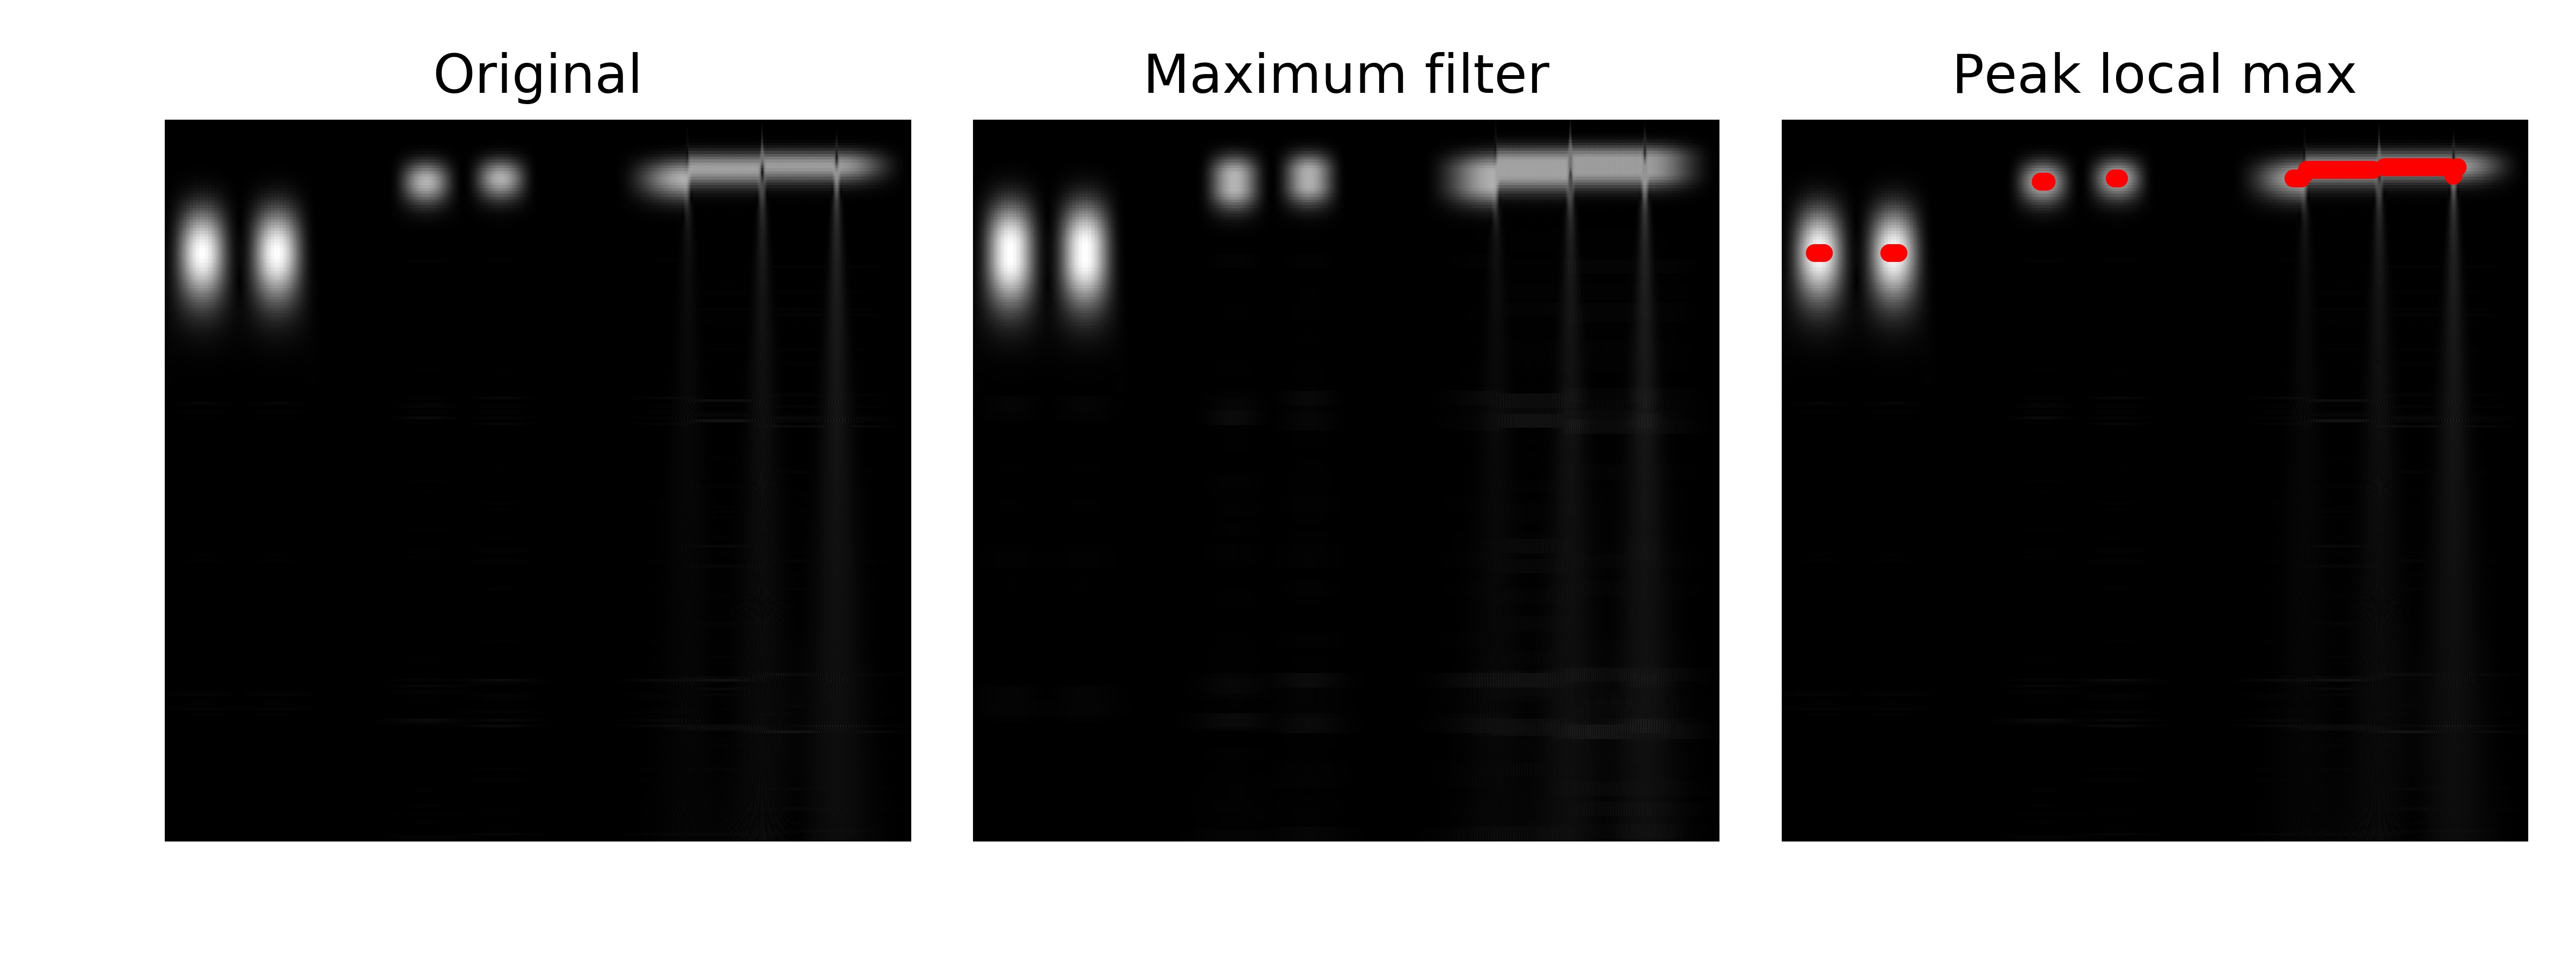
\includegraphics[width=\linewidth]{papers/autotune/sections/frames/images/cwtmaxima.jpg}
	\captionof{figure}{Die maxima Berechnung  der cwt}\label{fig:cwt_max}
\end{figure}%

In der Grafik \ref{fig:cwt_max} sieht man schön wie stabil die Frequenzen angezeigt werden. Auch wenn das Ergebnis der Koordinaten zurückgerechnet wird, kommt man auf die genaue Ursprungsfrequenz welche wir $x_{\text{Test}}$ zugewiesen haben. Sprünge, Anfangswerte und jegliche andere Unstetigkeit der Funktion verziehen das Ergebnis der cwt, jedoch bleibt dies vernachlässigbar.
\\

Die Grafik \ref{fig:stacked_max} bildet die Lokale Maximalstellensuche der Stacked-Frame-Analyse ab. Diese wurde auf die gleiche Art wie die \ref{fig:cwt_max} Analysiert und ausgewertet. Man kann auch hier die Frequenzen wieder zurück rechnen. Man sieht jedoch schon von Aug, dass die Resultate ein wenig schwanken. Beim Rückrechnen bekommt man dementsprechen auch schwankende Frequenzbänder. Da die Stacked-Frame-Analyse mit 48 Basen gemacht wurde sind die Schwankungen der Bänder noch so klein, dass die einzelnen Halbtöne von einander unterschieden werden können. Durch diesen Effekt ist es jedoch nicht möglich, eine Frequenz $f$ die 
\[f= fs\cdot 2^{\frac{1}{48}}\]  
von der gesuchten Frequenz zu unterscheiden. Folglich sollte man bei dieser Reckunstuktionsmethode, mindestens doppelt so viele Basen bereitstellen, wie Töne in einer Oktave gefunden werden möchten. 
\begin{figure}[!ht]
	\centering
	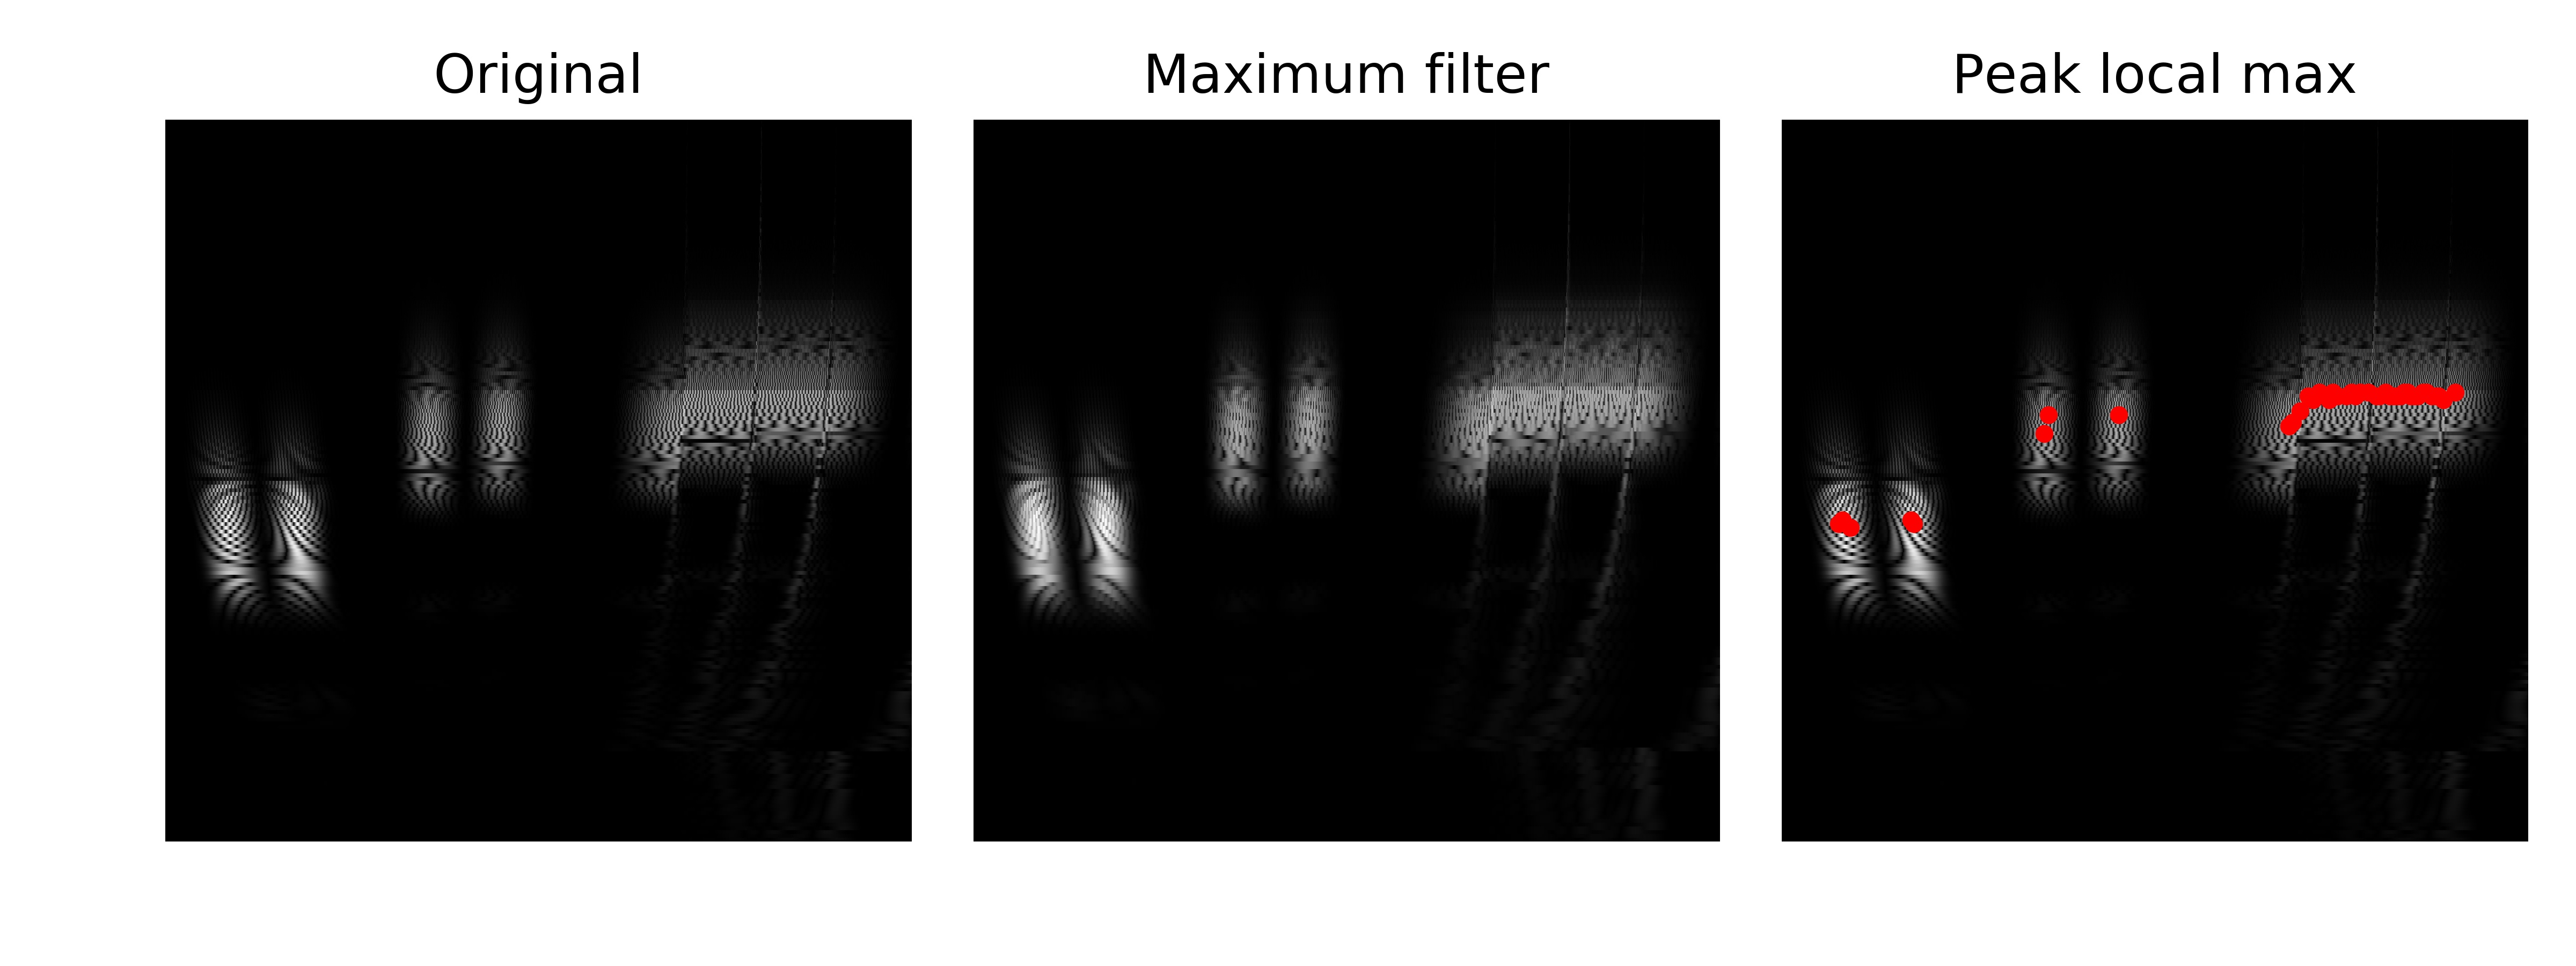
\includegraphics[width=\linewidth]{papers/autotune/sections/frames/images/Stacked/dwtmaxima.jpg}
	\captionof{figure}{Die maxima Berechnung  der Stacked-Frame-Analyse}\label{fig:stacked_max}
\end{figure}%


Bei der Overlaid-Frame-Analyse kann auf die selbe Art nach Maximalstellen gesucht werden. In der Abbildung \ref{fig:overlaid_max} können wieder sehr ähnliche Resultate, wie in den beiden voherigen Analysearten beobachtet werden. Die Rückrechnung gelingt auch wieder hier nur mit einem gewissen Fehler. Dieser kann jedoch mit der verwendung von mehr Basen minimiert werden.  Auch eine anschliessende Mittelung der Koordinaten die sehr nahe liegen verbessert das Resultat erheblich. Analog zu der Stacked-Frame-Analyse, benötigt man mindestens eine doppelte Anzahl Basen, wie Anzahl Töne in einer Oktave die gefunden werden möchten.
\begin{figure}[!ht]
	\centering
	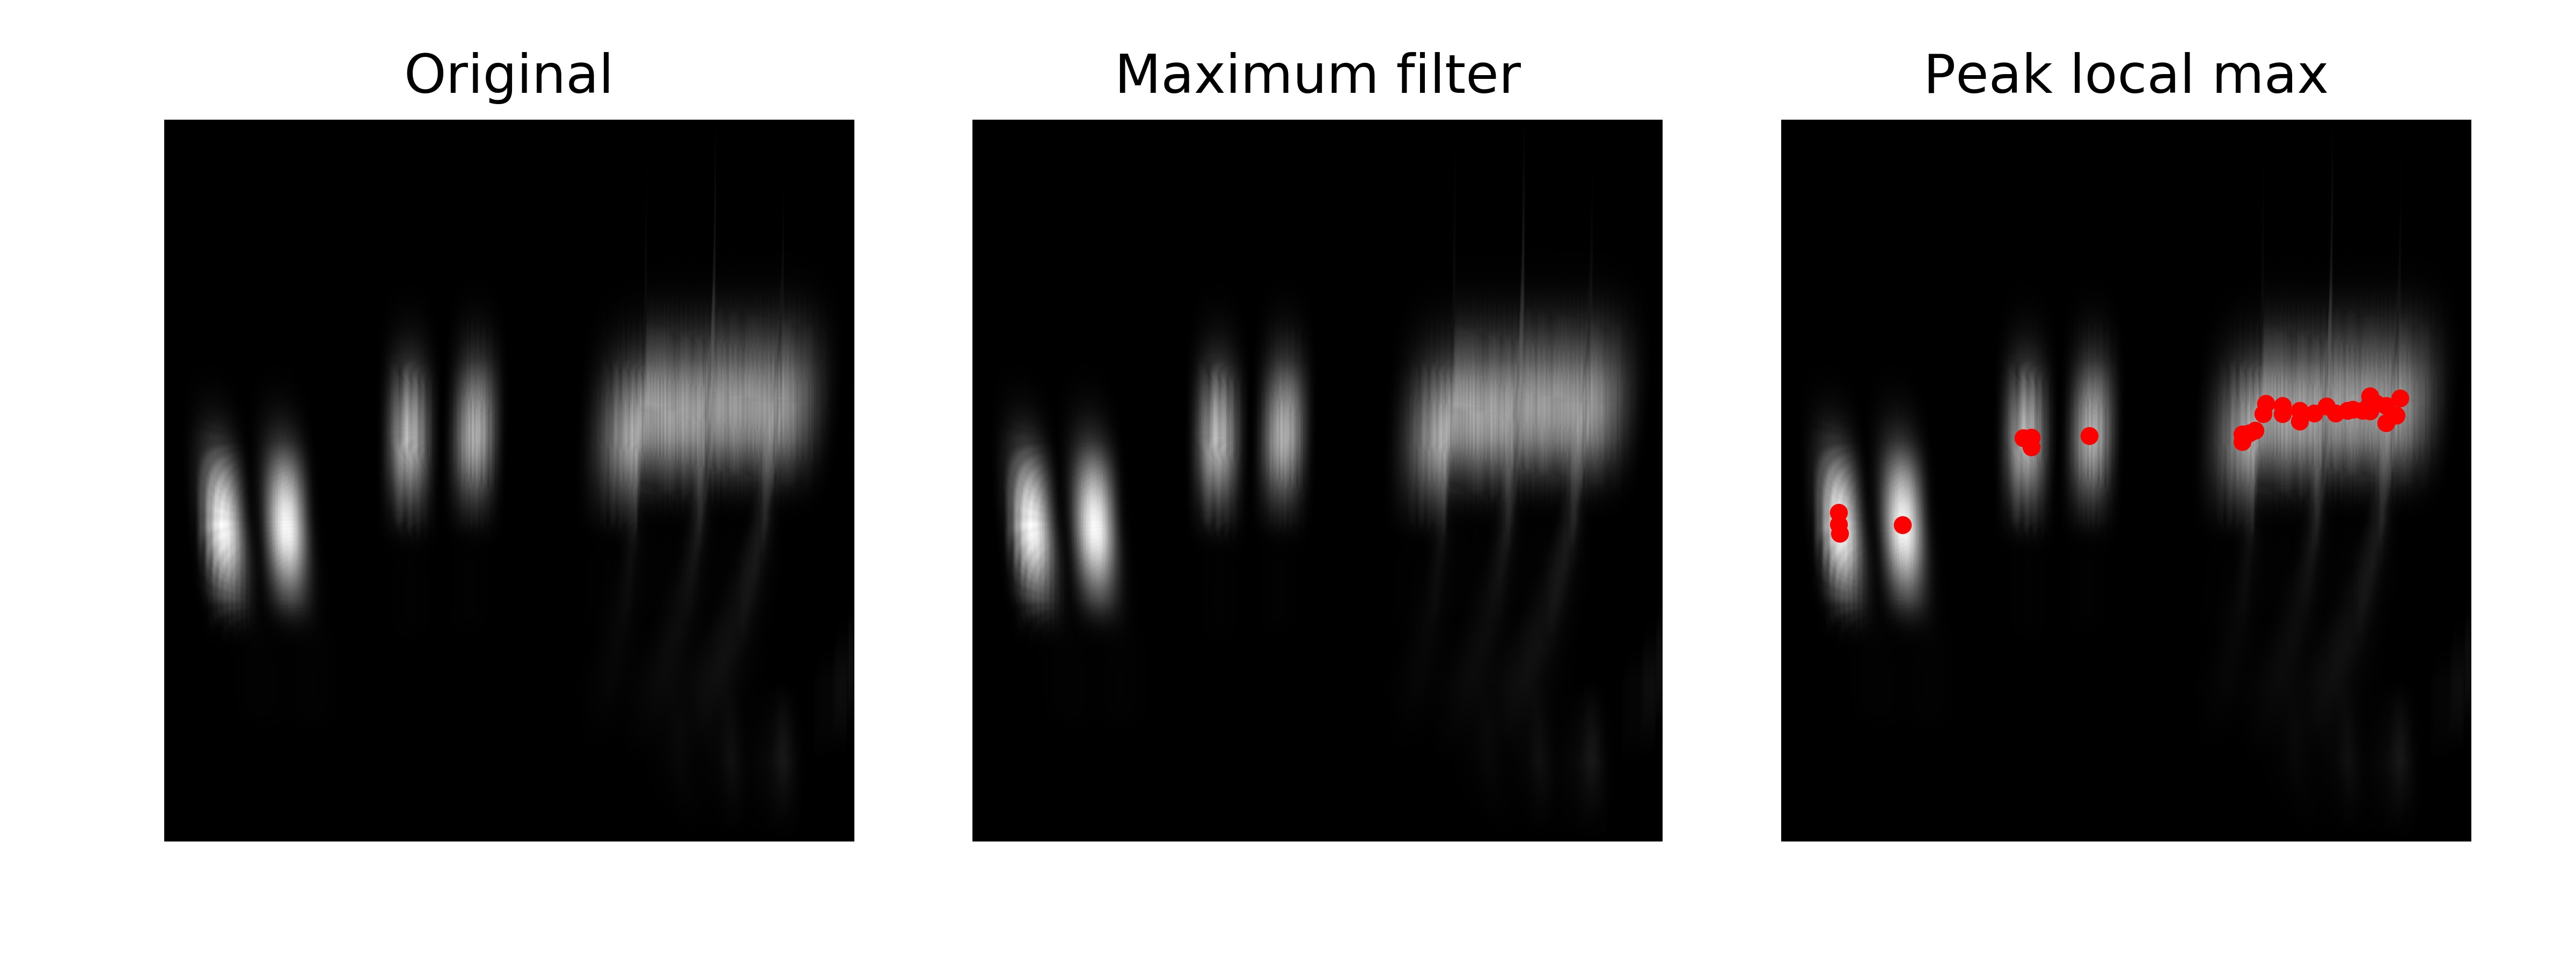
\includegraphics[width=\linewidth]{papers/autotune/sections/frames/images/Overlaid/dwtmaxima.jpg}
	\captionof{figure}{Die maxima Berechnung der Overlaid-Frame-Analyse}\label{fig:overlaid_max}
\end{figure}%

